\documentclass[a4paper,english]{report} 

\usepackage{fullpage}
\usepackage{subfig}
\usepackage[usenames,dvipsnames]{color}

%\def\documentstate{} % Lav om til FINAL når vi er done!
\usepackage[utf8]{inputenc}
\usepackage{fixme} % kræver at folk er smarte nok til at installere FiXme
\usepackage[T1]{fontenc}
\usepackage{babel}
%\usepackage{lmodern} % vector font, ikke bitmap!!
% ^- kun interessant med latex, pdflatex er vector i forvejen
\usepackage[final]{graphicx}
\graphicspath{{graphics/}}
\DeclareGraphicsExtensions{.pdf,.jpeg,.jpg,.png}
\usepackage{tikz}
\usetikzlibrary{positioning,shadows,arrows}

\usepackage{wrapfig}
\usepackage[final,plainpages=false]{hyperref}
\hypersetup{pdfborder=0 0 0} % Go away you ugly boxes!

\usepackage{amssymb}
\usepackage{amsmath}
\usepackage{verbatim}
\usepackage{multirow}
%\usepackage{subfig}
%\usepackage{slashbox}
%\usepackage{color}
\usepackage{listings}
\usepackage{listing}
\usepackage{algorithm}
\usepackage{algorithmic}
\usepackage[numbers]{natbib}

%\citestyle{chicago} % Chicago Manual of Style citations

%\renewcommand{\danishhyphenmins}{22} % fuck lorte orddeling!
\usepackage{ifdraft}
\ifdraft{
  \usepackage{draftwatermark}
  \SetWatermarkScale{4.0}
}{}

\setcounter{secnumdepth}{2}
\setcounter{tocdepth}{3}

%% default lst options

%% Special environments

\newenvironment{shcode}%
{\verbatim}{\endverbatim}

% use a TT font with bold 
\renewcommand{\ttdefault}{pcr}

\lstset{basicstyle=\ttfamily \footnotesize}
\lstset{keywordstyle=\textbf}
\lstset{commentstyle=\normalfont \textit}
\lstset{stringstyle=\bfseries}
\lstset{showstringspaces=false}

\lstset{frameround=tttt}
\lstset{frame=tLBr}

\lstnewenvironment{pythoncode}{\lstset{language=Python}}{}
\lstnewenvironment{cppcode}{\lstset{language=C++}}{}
% \lstnewenvironment{shcode}{\lstset{language=sh}}{}

%% Some commands
\newcommand{\todo}[1]{\textcolor{red}{#1}\fixme{#1}}

\newcommand{\class}[1]{\texttt{#1}}
\newcommand{\method}[1]{\texttt{#1}}
\newcommand{\file}[1]{\texttt{#1}}
\newcommand{\code}[1]{\texttt{#1}}

%%% Local Variables: 
%%% mode: latex
%%% TeX-master: "master"
%%% TeX-PDF-mode: t
%%% End: 


\newcommand{\reffig}[1]{figure \ref{#1}}
\newcommand{\refchapter}[1]{Chapter \ref{#1}}
\newcommand{\refsection}[1]{Section \ref{#1}}
\newcommand{\reflst}[1]{listing \ref{#1}}
\newcommand{\refalg}[1]{Algorithm \ref{#1}}

% Cite macroes
\newcommand{\chapterquote}[2]{
  \begin{quote}
    \raggedleft{
      \emph{#1}\\
      #2}
  \end{quote}
}

\newcommand{\citebook}[1]{\citep{#1}}
\newcommand{\quotebook}[2]{
  \begin{quote}
    \raggedright{\emph{#1}}\\
    \raggedleft{\citebook{#2}}
  \end{quote}}

\newcommand{\zhou}{Zhou et al.\citebook{1409079}}
\newcommand{\horn}{Horn et al.\citebook{1230129}}
\newcommand{\aila}{Aila and Laine\citebook{Aila2009}}

% Algorithm macros
\newcommand{\PARALLELFOR}[1]{\FOR{\textbf{each} #1 \textbf{in
      parallel}}}
\newcommand{\FOREACH}[2]{\FOR{\textbf{each} #1 \textbf{in} #2}}
\newcommand{\COMMENTIT}[1]{\STATE{\textit{\color{gray}// #1}}}
\newcommand{\PROCEDURE}[4]{\STATE{\hspace*{-1em}\textbf{procedure} #1 \\ 
    \hspace*{0.5em} \textbf{in} #2 \\ 
    \hspace*{0.5em} \textbf{out} #3 \\
    \hspace*{-1em}\textbf{begin} \\
    #4 \\
    \hspace*{-1em}\textbf{end}}}
\newcommand{\SYNC}{\STATE{\textbf{synchronize}}}
\newcommand{\ASSIGN}[2]{
  \STATE{#1 $\leftarrow$ #2}
}
\newcommand{\VAR}[1]{$#1$}
\newcommand{\DECLARE}[2]{\STATE{#1 : #2}}
\newcommand{\MIN}[2]{\textbf{min}$($ #1 , #2 $)$}
\newcommand{\MAX}[2]{\textbf{max}$($ #1 , #2 $)$}
\newcommand{\MOD}{\textbf{mod }}

% Math macros
\newcommand{\vectwoT}[2]{
  \left[#1, #2 \right]^T
}
\newcommand{\vecthree}[3]{
  \left[\begin{array}{c} #1 \\ #2 \\ #3 \end{array}\right]
}
\newcommand{\vecthreeT}[3]{
  \left[#1, #2, #3 \right]^T
}

%Tikz macroes
\tikzset{
  node/.style={circle, fill=white, draw, drop shadow},
  visitedNode/.style={circle, fill=green!40, draw, drop shadow},
  leaf/.style={rectangle, rounded corners=1mm, fill=white, draw, drop shadow},
  visitedLeaf/.style={rectangle, rounded corners=1mm, fill=green!40, draw, drop shadow}
}
\newcommand{\drawTri}[3]{
  \draw[fill=lightgray, drop shadow] (#1) -- (#2) -- (#3) -- (#1);
}
\newcommand{\drawAabb}[4]{
    \draw[dashed] (#1) -- (#2) -- (#3) -- (#4) -- (#1);
}
\newcommand{\drawRay}[2]{
    \draw[line width=0.5pt, dashed, ->] (#1) -- (#2);
}
\newcommand{\drawNode}[4]{
    \draw (#1) -- (#2) -- (#3) -- (#4) -- (#1);
}
\newcommand{\axes}[2]{
  \draw[->] (0,0) -- coordinate (x axis mid) (#1,0);
  \draw[->] (0,0) -- coordinate (y axis mid) (0,#2);
  %ticks
  \foreach \x in {0,2,...,#1}
            \draw (\x,1pt) -- (\x,-3pt)
		    node[anchor=north] {\x};
  \foreach \y in {0,2,...,#2}
     	    \draw (1pt,\y) -- (-3pt,\y) 
     		    node[anchor=east] {\y}; 

}

\newcommand{\shadowgraphics}[2]{
  \begin{tikzpicture}
    \node[rounded corners=1mm, drop shadow] {\includegraphics[#1]{#2}};
  \end{tikzpicture}
}


\begin{document}

\begin{titlepage}
\pagenumbering{alph}

\thispagestyle{empty}
\centering
    { \baselineskip=24pt
      \vspace*{80pt}
      %    {\LARGE Efficient algorithms for Ray Tracing Dynamic Scenes}\\
              {\LARGE Efficient Ray Tracing of Dynamic Scenes on the
                GPU} \\
              Master's Thesis
              \vspace*{20pt}
              \\
              \includegraphics[width=12cm,clip=true,trim=0cm 0cm 0cm 47pt]{sponzaShadow}
%              \includegraphics[width=12cm]{sponza2}
%              \shadowgraphics{width=12cm}{sponza2}
              \vspace*{40pt}
              \\
              \begin{minipage}{0.4\textwidth}
                \centering
                Asger Dam Hoedt \\ asgerhoedt@gmail.com \\ 20051770
              \end{minipage}
              \begin{minipage}{0.4\textwidth}
                \centering
                Thomas Sangild Sørensen \\ sangild@cs.au.dk
              \end{minipage}
    }
    \vfill
    \small
    Department of Computer Science\\
    Aarhus Universitet
\end{titlepage}

\clearpage\pagenumbering{Roman}

%% Isbrief:200-300words. 
%% • Summarizes your work:
%% – What problem does this paper solve?
%% – Why is this problem important for medical image computing (the context and motivation)? 
%% – How does your method work? 
%% – How does it differ from previous work? 
%% – How much better than previous work is it?
%% • There are usually no references in the abstract
%% • The abstract should be readable and understandable by non-experts


\begin{center}
\begin{minipage}{0.7\textwidth}
\section*{Abstract}

This thesis is aimed at raytracing dynamic scenes and doing that efficiently
while harnesing the massive power of todays graphics cards. It is motivated by
the ever increasing interest in raytracing and global illumination for creating
effects in movies, but also the increased usage of 2D and 3D ray tracing in
modern computer games.

The thesis explores different techniques for creating hierarchical ray tracing
acceleration structures, specifically the binary kd-trees, and how to create
these efficiently on graphics hardware.

\fixme{Quality is defined as ray tracing speed}

While previous work with kd-trees has focused on creating optimal acceleration
structures, the goal of this thesis is to explorer the tradeoffs between
spending time producing structures of high quality or more quickly produce a
lower quality acceleration structure. This tradeoff can be very important in
dynamic scenes, where the acceleration structure may have to be rebuild for
every frame.

As part of the thesis an optimized ray tracer will be developed to evaluate the
quality of the kd-trees produced and to estimate if there is a potential
performance gain to be had by quickly producing kd-trees of lower quality.

\end{minipage}
\end{center}

% Show that to achive raytracing of dynamic scenes, focus should not
% be on creating 'optimal' trees, but instead on creating good trees
% fast.






% Efficiently create KD trees on the GPU and ray trace them.

% KDtree focus will be on optimizations and the tradeoff between
% spending extra time on the kd-tree instead of ray tracing.




\tableofcontents

\clearpage\pagenumbering{arabic}


%\maketitle

%% • The introduction must be dynamite. 
%% – The reader forms an oppinion of the work right from the start... 
%% • The introduction is an extension of the abstract. 
%% • Should be easy to read and understand 
%% • Should make it easy for anyone to tell
%% – What your paper is about 
%%   – What problem it solves
%%   – Why the problem and solution is interesting and relevant (motivation and context). Is it a long- outstanding problem?
%%   – What is new in your paper and how (much) does it improve on the strongest alternatives/previous work (include a few of the most relevant references here).

%% • Start the introduction with the motivation. Think in large contexts and don’t be afraid to be a poet.
%% • All implications, contributions and keypoints of your work must be included here.
%% • Make it very clear how your work will impact the future of Realistic image generation (will people use it?).
%% • If your work is pioneering, s-p-e-l-l i-t o-u-t.
%% • Briefly make it clear how you evaluate your method in the Results section.
%% • Make sure to explain where your method applies and where it does not apply (limitations).


\chapter{Introduction}

\chapterquote{Focus is a matter of deciding what things you're not
  going to do.}{John Carmack}


% Motivation

\textit{Rendering} is the process of converting a scene description into an
image and lies at the heart of \textit{computer graphics}. The ability to render
complex scenes realistically or distinctly is vital in several areas; computer
games, movies and even medical imaging. A scene is made up of models, which can
consist of several thousand geometric primitives, usually triangles. \fixme{Kan
  dette gøres mere læsevenligt?}Information about these triangles are stored at
the vertices and can be its position, a normal perpendicular to its surface or
its color among other things. Such information stored at a triangle's vertices
are called \textit{vertex attributes}.


% Rasterization and cube mapping

When real-time rendering is needed, the technique of choice for the last one and
a half decade has been \textit{rasterization}. In rasterization a geometric
primitive's vertex attributes are mapped onto a \textit{raster}\footnote{A flat,
  2D grid.} and used to calculate the color of individual raster cells. This
technique is so popular in the gaming industry that processing units were
created specifically for rasterization, the \textit{Graphics Processing Unit} or
\textit{GPU} for short. Due to the industry's ever increasing demand for more
detailed models and visual effects, the GPUs have seen a massive increase in
both computational power and memory bandwidth over the last
decade. Unfortunately, even with all this power, certain aspects of rendering are
still not easily solved by rasterization. \textit{Reflection} and
\textit{refraction} effects on non-flat surfaces are still notoriously hard to
recreate. The reason is that the reflection of complex objects can not easily be
mapped to a two dimensional grid, such as the raster. Reflections of complex
objects can be approximated by \textit{environment mapping} or \textit{cube
  mapping}, of which a short describtion can be found on \reffig{fig:cubemap}. A
problem with cube mapping is that the scene must to be rendered once for each
side of the cube map, which increases the cost of rendering a scene
drastically. Another shortcoming of cube mapping is that it doesn't support
\textit{self reflection}, since it is only the surrounding environment that is
rendered onto the map.

\begin{figure}
  \centering
  \includegraphics{Cube_mapped_reflection_example}

  \vspace{3mm}
  \parbox{9.5cm}{\caption[Cube mapping visualized.]{A visualization of cube
      mapping. The environment is rendered onto the sides of the cube and then
      mapped onto the object inside the cube map. The mapping is performed by
      using the calculated reflection vector as an index into the cube
      map.\\Image from
      http://en.wikipedia.org/wiki/Reflection\_mapping}\label{fig:cubemap}}
\end{figure}

% Ray tracing and comparing it to rasterization

An alternative to rasterization is \textit{ray tracing}, which elegantly solves
reflection and refraction by tracing rays from the viewer's eye and into the
scene, spawning and tracing new reflection- and refraction rays as needed when
geometry is intersected. A comparisson of cube mapping and ray tracing is given
in \reffig{fig:reflectingDragons}, where I have rendered a reflecting Stanford
Dragon using both techniques. Notice how the ray traced dragons backside
reflects its neck, while the cube mapped version only reflects the surrounding
box. Advanced lighting techniques that produce photorealistic images are also
based on ray tracing. One such technique is \textit{photon mapping}, which can
accurately reproduce the effects of light bouncing of reflective surfaces,
caustics and color bleeding.

\fixme{Write something about how all figures are my own unless explicitly
  stated!}

\begin{figure}
  \centering
  \subfloat[A cube mapped reflecting dragon.]{
    \includegraphics[width=7cm]{cubemappedDragon}
    \label{fig:cubeDragon}
  }
  \hspace{10pt}
  \subfloat[A ray traced reflecting dragon. Notice the self reflection
    on the back and inside the mouth.]{
    \includegraphics[width=7cm]{semiReflectingDragon}
    \label{fig:rayReflectingDragon}
  }
  \caption[Reflections created with cube mapping and ray tracing.]{An example of
    the difference between using cube mapping or ray tracing for
    reflections.}
  \label{fig:reflectingDragons}
\end{figure}


% High cost used to make it unattractive for interactive scenes.  What I will
% show, doing it dynamically, which is interesting for games and movie
% development

The increased realism that can be achieved by using ray tracing does come at a
high computational cost, which has previously made it unattractive for
interactive applications or dynamic scenes. Nonetheless, the continued increase
in computational power of both CPUs and GPUs, coupled with research into the
area of \textit{interactive ray tracing}, has yielded some remarkable results.
Scenes of approximately 100k triangles can now be ray traced in real-time, even
with effects such as shadows, reflection and refraction added. This makes ray
tracing an increasingly more interesting alternative to rasterization. In this
thesis I will examine \textit{ray tracing of dynamic scenes}, with the express
goal to minimize the time between modifying the scene and presenting a user with
visual feedback of the change. This would be very interesting in the film
industry, where ray tracers are used to create
\textit{CGI}\footnote{Computer-generated Imagery} effects and 3D artists need
fast visual feedback while modifying the scene.

%% In this thesis I will examine \textit{ray tracing of dynamic scenes}, which is
%% becoming an interesting alternative to rasterization in the gaming industry in
%% the years to come. The film industry has also used ray tracing to do their
%% \textit{CGI}\footnote{Computer-generated Imagery} effects for quite some time,
%% and for the 3D artists working on these effects, it would certainly be
%% beneficial to use a ray tracer that is able to produce fast visual feedback,
%% when an artist rearranges the scene.

% We need Acceleration stuctures for ray tracing to achieve this

To improve the performance of ray tracers, several acceleration structures have
been developed. The most popular structures are \textit{hierarchical data
  structures}, such as trees, and ray tracers that traverse these are called
\textit{hierarchical ray tracers}. When a ray traverses a hierarchical data
structure it is in search of the nearest leaf node, which contains references to
the geometry nearest to the ray. If the ray finds that it did not see, or
\textit{intersect}, any of the geometry in the current leaf node, it advances
beyond that leaf and performs another traversal of the structure.

The structure employed in this thesis is the \textit{kd-tree}, a binary, space
partitioning tree-structure, which recursively subdivides $k$-dimensional
geometry by splitting it with an \textit{axis aligned splitting plane}. Each
interior node in the tree contains a splitting plane and a reference to the
location of its left and right children, while the leafs contain references to
the geometry associated with them.
%% An example of a subdivided scene and the corrosponding tree can be seen on
%% \reffig{fig:kdIteration} in \refchapter{chp:kdTrees}, where kd-trees will be
%% introduced thoroughly. 
If a leaf node is split by a splitting plane, the geometry associated with that
leaf must be associated with its two newly constructed child nodes. The quality
of a kd-tree is defined as the ease with which it allows a scene to be ray
traced and is affected by the choice of splitting planes. A lot of computational
power can go into finding optimal splitting planes, as there are infinitely many
possible \textit{splitting plane candidates}, or \textit{split candidates}, to
consider.

%% In a high quality kd-tree, splitting planes have been chosen such that
%% spatially close geometry are allocated into the same subtree and the scene
%% can be ray traced as fast as possible. Choosing a splitting plane for a node
%% is the topic of \refsection{sec:splittingPlane}.

In order to facilitate dynamic scenes, the data structure must also be
dynamic. It is possible to dynamically add and remove elements to a kd-tree, but
doing so can degrade the quality of the kd-tree or its subtrees. If a subtree's
quality has degraded too much, it will have to be reconstructed to again
facilitate fast ray tracing. In the worst case scenario this reconstruction
needs to be performed on the entire tree and is equivelant to a complete
reconstruction. Because of this, the algorithms for creating and restructuring
kd-trees needs to be very fast, and might even have to sacrifice tree quality
for improved construction speed. This tradeoff between speed and quality is also
what makes dynamic scenes interesting compared to static scenes. Ray tracers
rendering static scenes can use as much time as needed to produce acceleration
structures of high quality. This may not be possible in dynamic scenes, where a
user that modifies the scene will want visual feedback of the modifications made
as fast as possible.

In general there are three ways to optimize ray tracing with respect to dynamic
scenes to achieve maximum efficiency:

\begin{enumerate}
  \item \textbf{Building a higher quality acceleration structure -} An
    acceleration structure of higher quality will reduce the time it takes the
    ray tracer to find the nearest intersecting point between a ray and the
    scene. Algorithms for producing kd-tree's of different quality is the topic
    of \refsection{sec:splittingPlane}.
  \item \textbf{Build the acceleration structure faster -} As described above,
    the acceleration structure may need to be entirely reconstructed each time a
    dynamic scene is rendered. Being able to rebuild it fast is therefore
    crucial. One way to ensure a faster reconstruction is by reducing the time
    spent deciding where to place the splitting plane, which can result in trees
    of lower quality.
  \item \textbf{Create a faster ray tracer -} Several optimizations exist that
    improve the speed of a ray tracer without modifying the underlying
    acceleration stucture. Such optimizations will be discussed in
    \refsection{sec:hierarchicalTraversal}.
\end{enumerate}


% Why do it on the GPU, yes why indeed? Leaves the CPU free to do
% other things than rendering.

As observed at the beginning of this chapter, GPU's have grown quite powerful
over the last decade, and since the introduction of programmable GPU's and
NVIDIA's \textit{CUDA}\footnote{Compute Unified Device Architecture.}
framework, many algorithms have been succesfully ported to utilize the resources
of the GPU. In this thesis I too will use the massive computational power of the
GPUs to accelerate the creation of data structures and ray tracing them. The
most compelling reason to do this, is that it leaves the CPU free to handle
other aspects of a graphics application, such as game logic and networking
communication.

%% However, the results achieved in this thesis with respect to ray tracing dynamic
%% scenes are architecture independent and apply to the CPU aswell as the GPU.

\chapter{Previous Work}

\chapterquote{If you want to make an apple pie from scratch, you must
  first create the universe.}{Carl Sagan}

% Raytracing work


% KD-tree work


% Data structures

% Previously constructing the KD-tree was most effective on the CPU,
% optimized and fast for multi core CPU's
\citebook{1230129}

% GPU solutions had to use other datastructures such as grids
\citebook{844181}

% or create hybrid GPU/CPU solutions
\citebook{1572783}

% Recent research has made it possible to construct KD-trees
% efficiently on GPGPU's
\citebook{1409079}

% Aila has looked at persistent threads to accelerate raytracing. In
% this thesis I will utilize their idea to accelerate the SAH
% calculations of individial nodes.
\citebook{Aila2009}


\section{Goals}

In this thesis the goal is not to produce images of photorealistic quality, or
create an interactive ray tracer \footnote{This goal alone can be achieved
  trivially by reducing the complexity of the ray traced scene or lowering the
  image resolution.}. Instead this thesis will explorer ray tracing acceleration
structures, specifically the kd-tree, and its impact on ray tracing efficiency
for dynamic scenes.

The main topic in this thesis is the relationship between the time spend
constructing a kd-tree and its resulting quality, i.e. how fast can it
accelerate ray tracing. Building on the kd-tree implementation presented by
\zhou{}, I will investigate different parts of the kd-tree construction phase
for dynamic scenes and whether it is worthwile in dynamic scenes to sacrifice
tree quality to gain faster kd-tree construction. The two parts of the kd-tree
creation phase that will be investigated is the choice of splitting plane and
how geometry is associated with child nodes after a split. As part of this
investigation I will describe several different solutions and show how to
implement them efficiently on dataparallel GPUs using CUDA.

The kd-trees created by the different methods above will be evaluated by how
fast they can be constructed and how efficiently a ray tracer can traverse them
to render a scene. During evaluation I will always perform a complete rebuild of
the kd-tree before rendering a scene. This is done to ensure that my tests
capture the worst case scenario for dynamic scenes, which is a complete update
of the entire scene and thus a complete rebuild. The goal of this thesis is then
to find a kd-tree configuration that minimizes the total time spent both
recreating and traversing the acceleration structure and evaluate the tradeoff
between construction speed and tree quality.

I will furthermore discuss the ray tracers used to evaluate the quality of the
kd-trees. To provide a fair and useful comparison of a kd-tree's construction
time and its quality, I will need to create a highly optimized ray tracer. These
optimizations are important as a fully optimized ray tracer can render scenes up
to 70\% faster than a basic implementation and does so independent of the
underlying kd-tree and its construction schemes. While I will be discussing and
applying these optimizations, such as the short-stack optimization from \horn{},
the topic is secondary to kd-trees and merely included for evaluation purposes.

Given the added overhead of continuously rebuilding the kd-trees, an interesting
question is whether or not we even need them. I therefore present an
\textit{exhaustive ray tracer}, which does not use any acceleration structure
and thus intersects every ray with every triangle. The exhaustive ray tracer
will be compared to the hierarchical ray tracers and hopefully motivate the
continued use of acceleration structures for dynamic scenes.

\section{Overview}

The rest of the thesis is structured as follows:

% Previous work

%% The next section details previous work in the area of ray tracing and
%% kd-tree construction. This includes a brief history of when ray
%% tracing was introduced, aswell as key points in time for different
%% acceleration structures. The last part of this section will focus on
%% kd-trees and ray tracing on graphics hardware. Changes in this thesis
%% compared to previous work in the area are also outlined in this
%% section.

% Understanding CUDA

\refchapter{chp:GPGPU} introduces NVIDIA's CUDA framework. Here I will describe
its thread and memory model. I will then go on to describe a new primitive
proposed by \sengupta{}, which will be needed, e.g. when assigning triangles to
child nodes after their parent node has been split. The last part of this
chapter will focus on optimization techniques specific to CUDA and apply these
incrementally in a case study of a global minima algorithm.

% kd-trees

\refchapter{chp:kdTrees} is devoted to discussing the construction of
kd-trees. The first part of this section deals with the general kd-tree
construction algorithm. Here I will present several algorithms for choosing the
splitting plane and discuss three different approaches used to associate
triangles with leaf nodes. The second part of \refchapter{chp:kdTrees} deals
with the actual implementation of kd-trees on a GPU and will describe how the
nodes are structured in memory and how to construct binary trees effectively on
dataparallel hardware.

% ray tracing

Having introduced kd-trees, \refchapter{chp:rayTracing} will deal with the
algorithms for traversing such trees and ray tracing a scene. Here several
optimizations to a basic hierarchical ray tracer will be discussed and
incrementally added. First though, an exhaustive ray tracer is presented and
will be used in teh Conclussion to motivate the use of hierarchical data
structures. This chapter also includes a discussion of two triangle intersection
algorithms with respect to achieving maximal performance on GPUs.

% Results

In \refchapter{chp:results} I will first evaluate the performance of several
different ray tracers. I will then use the ray tracer that generally performs
best to evaluate the quality of the different kd-trees created. The metric used
to determine which kd-tree construction algorithm performs best will be the
total rendering time, i.e. the sum of the construction time and ray tracing
time.

% Conclusion % Future work

I will then conclude my work by discussing my results and their implications for
the future of ray tracing dynamic scenes. Finally in \refchapter{chp:future} I
will address future improvements based on the experience I have gained while
working on this thesis.



\chapter{Previous Work}

\chapterquote{If you want to make an apple pie from scratch, you must
  first create the universe.}{Carl Sagan}

% Raytracing work


% KD-tree work


% Data structures

% Previously constructing the KD-tree was most effective on the CPU,
% optimized and fast for multi core CPU's
\citebook{1230129}

% GPU solutions had to use other datastructures such as grids
\citebook{844181}

% or create hybrid GPU/CPU solutions
\citebook{1572783}

% Recent research has made it possible to construct KD-trees
% efficiently on GPGPU's
\citebook{1409079}

% Aila has looked at persistent threads to accelerate raytracing. In
% this thesis I will utilize their idea to accelerate the SAH
% calculations of individial nodes.
\citebook{Aila2009}


\chapter{Understanding the GPGPU}\label{chp:GPGPU}

\chapterquote{Hardware: The parts of a computer system that can be
  kicked.}{Jeff Pesis}



% Motivate the use of GPUs

Because of the evergrowing demand for new effects and more detail in
computer games and other 3D graphics applications, GPU's have seen a
massive increase in power over the last decade, as evidenced by
\reffig{fig:gflops}. A similar figure comparing the theoretical
throughput of GPU's and CPU's can be seen in \citebook{CUDAPG}. With
this in mind it is easy to understand why one would want to perform
ray tracing entirely on the GPU.

\begin{figure}
  \centering
  \includegraphics[width=8cm]{GFLOPS}
  \caption{A comparison of the development of floating point
    operations pr. second on GPU's and CPU's. \\The figure is borrowed
    from Chapter 1 in \citebook{CUDAPG}}.
  \label{fig:gflops}
\end{figure}

% What is different form CPUs

Utilizing all this power effectively, however, is not straightforward
and in order to create algorithms on the GPU that run faster than their
CPU counterparts, we need to understand how the GPU works.

The reason behind the difference in theoretical throughput seen in
\reffig{fig:gflops}, is that the CPU is designed for handling all
kinds of problems, with a large cache at it's disposal and efficient
handling of control flow. The GPU on the other hand is designed for
high throughput of small, arithmetically intense, \textit{dataparallel
  programs}\footnote{Each processor performs the same instruction
  concurrently on multiple data elements.}, which is exactly what is
required of a graphics card processing thousands of independent
vertices and performing the same shading on hundreds of thousands of
color fragments.

Since the graphics card is designed to perform vertex and fragment
processing independently of their respective neighbouring threads,
this also means that when programming the graphics card, no
assumptions can be made about which thread is where in it's
execution. This presents a problem in cases where the $n$'th thread
depends on information from all previous $n-1$ threads, fx when
splitting data or calculating the minimum or maximum values of $N$
vertices. NVIDIA's CUDA remedies this somewhat by providing
synchronization commands, but since these will only synchronize a
subset of the running threads, the overall problem remains the same.

% Why not use GPU/CPU solutions

An obvious solution is ofcourse to perform easily parallisable
operations on the graphics card and leave the rest for the
CPU. However, the following quote comes to mind:

\quotebook{
  It is important to include the overhead of transferring data to and
  from the device in determining whether operations should be
  performed on the host or on the device.
}{CUDABPG}

So once it has decided to use the graphics card, one cannot simply
transfer data back to the CPU in order to perform some operation and
then transfer it back the GPU. The overhead would in many cases be too
large to see any performance increase at all.

%% Fortunatly Sengupta et al. has come up with a solution to the
%% scattering problem, which will be discussed further in
%% \refsection{sec:GPUprims}.


% Overview of the chapter

Finding effective GPGPU solutions to the above mentioned problems is
the motivation for this chapter, which is structured as follows.
First we shall take a look at the how threads and memory is organized
on the graphics card. Understanding this will be critical in
developing GPGPU efficient solutions. Then a section will present new
GPGPU scan primitives, which will help us to perform data scattering
and reductions on dataparallel hardware. I will then be discussing a
couple interesting optimization techniques on the GPGPU, while
applying them to a reduction case study.



\section{The Architecture of the GPGPU}

To understand the architecture of the GPGPU, we must first understand the
relationship and layout of threads and then the different kinds of
memory available to threads.

\subsection{Thread Model}

% Grid, blocks, warps and threads. We will only deal with the one
% dimensional case.

The graphics card is able to handle execution of more than a million
threads sequentially. Simply considering a graphics application
running at a 1440x900 resolution should convince anyone of this. While
above I have argued that all of these threads are executed
independently of each other, NVIDIA's CUDA architecture does place
these threads in a hierarchy, which provides programmers with some
control over thread execution.

At the lowest level threads are scheduled and executed completely
parallel in small groups called \textit{warps}\footnote{The term
  originates from weaving, the first parallel thread
  technology.\citebook{CUDAPG}}, usually with a warpsize of 32. While
threads in a warp have their own instruction counter and register
state, and therefore logically can branch independently of
neighbouring threads, a warp can only execute one specific instruction
at a time. The following example should help clarify this.

\begin{algorithmic}
  \IF{threadID < 16}
    \ASSIGN{$x$}{$threadID$}
  \ELSE
    \ASSIGN{$x$}{$32 - threadID$}
  \ENDIF
\end{algorithmic}

The first 16 threads in the warp will evaluate to true and thus
perform the assignment $x \leftarrow threadID$, while the next 16
threads will evaluate to false and execute the alternate statement $x
\leftarrow 32 - threadID$. Since the warp can only perform one
distinct instruction at a time, it will have to first execute $x
\leftarrow threadID$, leaving the last 16 threads idle. It next
executes the else branch, meaning the first 16 threads are left
idling. While this example shows how branching can hurt performance,
when all threads in a warp do not take the same execution path,
knowning that all threads in the warp always are synchronized can also
be very beneficial, as will be shown in
\refsection{sec:loopUnrolling}.

\begin{figure}
  \centering
  \includegraphics[width=8cm]{ThreadLayout}
  \caption{A figure of CUDA's thread layout.\\ The figure is borrowed
    from Chapter 2 in \citebook{CUDAPG}}.
  \label{fig:gflops}
\end{figure}


% It is a wide SIMD/SIMT, Single-Instruction / Multiple-Thread,
% machine. This means branching hurts. Alot!


\subsection{Memory Model}

\subsubsection{Global Memory}

% Slow, coalescene of data types with size 1, 2, 4, 8, and 16 bytes.

% Coalesced memory access, float4 instead of float3

% The alignment requirement can be forced: stuct __align__(8) {

% Mention textures and cache. The project developed for this thesis
% will not be using textures, since global memory also has cache as of
% 2.0 hardware.

\subsubsection{Registers and Local Memory}

Kernel variables that the compiler will most likely place in local memory are:

\begin{itemize}
  \item Any array that from the compilers point of view are dynamically indexed.
  \item Structures or arrays that are to large to fit inside registers.
  \item Any variable in the kernel, if the kernel has to many
    variables to place them all in register memory. This is referered
    to as \textit{register spilling}.
\end{itemize}

% Combat local memory by using launch bounds

\subsubsection{Shared Memory}

% Faster than global/local

% Used to overcome the limitations of global and local memory.

% Can be used as global cache on never CUDA architectures isntead of
% textures and shared mem. nice we laike

% Bank conflicts, nothing is ever as good as it seems.




% NVIDIA mentioned 3 optimization points

% Structures of arrays vs arrays of structs. Usefull when fx
% sorting. CUDPP article/forum. Plus cache performance.

% Unrolling loops, even when it means more work. Preprocess lower
% nodes yields nearly a 50% speedup from this.


\section{Wide SIMT primitives}\label{sec:GPUprims}

% Scan and compact

% cite sengupta paper

\quotebook{...efficient solutions to parallel problems in which each
  output requires global knowledge of the inputs.}{Sengupta:2007}

% Useful for scattering data

% Give array example

\section{Optimization Techniques}

% Naive implementation

\section{Case Study: Reduction}

\subsection{Switching to shared memory}

% Does that make any difference on 2.0 archs?

\subsection{Using Registers}

% Storing the thread local result in both smem and register

\subsection{Loop unrolling}\label{sec:loopUnrolling}

% Unroll the loops.

% Then move the first up to where data is loaded into shared mem

% And move the last reduction down where the final result is written.




%\section{Case Study: Segmented Reduction}

% Alot of reductions and iterative algorithms. It is therefore
% important to know how to optimize these from a naive implementation.

% Algorithm from bla

%\subsection{Naive implementation}

%\subsection{Switching to shared memory}


%\subsection{Rewriting slow math operations}

% Pow is 'expensive' and can be replaced by a simple doubling of the
% indices.

%\subsection{Unrolling the loops}

% Can be done with a template parameter. Would still need to check
% range, but could remove the loop variables. Would need a few speciel
% cases for small kernelsizes (1 - 4 threads).

% Pros

% Shared memory is almost halved

% Only needs half the threads

% No dummy variables

% Cons

% Unrolling yields more instructions for executions that would only
% loop once. However since that only account for the last couple of
% nodes, it is more than made up for by all the previous
% nodes. Version 2 could be used for executions with 2 or less threads.

% Unrolling must also adds a check for out of bounds (or replaces the
% loop with that check) However making sure that single block bounding
% box reductions are never brought to the segmented reducer will
% ensure at least 2 values exist and one bounds check can be omitted.


\chapter{KD-Trees}\label{chp:kdTrees}

%% \chapterquote{In theory, there is no difference between theory and
%%   practice. But, in practice, there is.}{Jan L. A. van de Snepscheut}

\chapterquote{With todays's fast ray tracers, the difference between a
  ``good'' and a naïvely built kd-tree is often a factor of 2 or
  more.}{Ingo Wald and Vlastimil Havran}

\fixme{Anden argumentation for kd-træet? Fjern distance tests?}

% About KD-trees

Before we in \refchapter{chp:rayTracing} discuss how rays will
traverse the kd-tree, we must first examine the structure of it and
how it is created.

% Why KD tree compared to other structures

As mentioned earlier in this thesis, kd-trees was chosen as the data
structure employed to accelerate ray tracing. This choice is based on
several factors.

% Cheap intersection / distance to tests. Havran p. 51

One of them is the ease with which the signed distance, $t$, from a
ray to a kd-trees axis aligned splitting plane can be computed. In
\refsection{sec:hierarchicalTraversal} we shall see that this distance
is essential to traversing the tree. An axis aligned splitting plane
is described by an axis, $d \in \{x, y, z\}$, and it's position along
that axis, $N_d$. The signed distance from any ray, $R(t) = O + tD$,
to the splitting plane is then simply calculated as

\begin{displaymath}
  t = \frac{N_d - O_d}{D_d}
\end{displaymath}

For comparison a generel \textit{binary space partition} tree,
\textit{BSP} tree, with arbitrarily oriented splitting planes, given
by $ax + by + cz + d = 0$ has a much more complex distance function.

\begin{displaymath}
  t = \frac{a O_x + b O_y + c O_z + d}{a D_x + b D_y + c D_z}
\end{displaymath}

\fixme{Drop bounding volumes?}

It becomes even more complex when bounding volumes are used. An axis
aligned bounding box can be described by 2 points, $V_{min}$ and
$V_{max}$. Calculating the signed distance to any rays entry and exit
point is then

\begin{displaymath}
  \begin{array}{l}
    t_{near,d} = min((V_{min,d} - O_d) / D_d, (V_{max,d} - O_d) / D_d)\\
    t_{entry} = max(t_{near,x}, t_{near,y}, t_{near,z})
  \end{array}
\end{displaymath}

The distance from the ray origin to all of the bounding box sides are
calculated, then the minimum along each axis is chosen and the maximum
of these values are the distance to the entry point. The distance to
the exit point is calculated similarly.

\begin{displaymath}
  \begin{array}{l}
    t_{far,d} = max((V_{min,d} - O_d) / D_d, (V_{max,d} - O_d) / D_d)\\
    t_{exit} = min(t_{far,x}, t_{far,y}, t_{far,z})
  \end{array}
\end{displaymath}


If the rays exit distance lies closer than the entry distance, then
the ray did not intersect the bounding volume, an example of this is
given on \reffig{fig:rayBoxIntersection}.

\begin{figure}
  \centering
  \subfloat[Ray miss.]{
    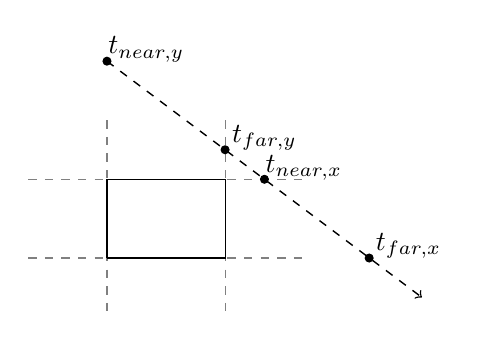
\begin{tikzpicture}[y=0.5cm, x=.5cm,font=\sffamily]
      % Planes
      \draw[dashed, color=gray] (-2,0) -- (5,0);
      \draw[dashed, color=gray] (-2,2) -- (5,2);
      \draw[dashed, color=gray] (0,3.5) -- (0,-1.5);
      \draw[dashed, color=gray] (3,3.5) -- (3,-1.5);

      % AABB
      \draw (0,0) -- (3,0) -- (3,2) -- (0,2) -- (0,0);

      % Ray
      \drawRay{0,5}{8,-1}

      % Intersection
      \draw[fill=black] (0,5) circle (0.05cm);
      \draw (1,5.3) node{$t_{near,y}$};
      \draw[fill=black] (3,2.75) circle (0.05cm);
      \draw (4,3.05) node{$t_{far,y}$};
      \draw[fill=black] (4,2) circle (0.05cm);
      \draw (5,2.3) node{$t_{near,x}$};
      \draw[fill=black] (6.66,0) circle (0.05cm);
      \draw (7.66,0.3) node{$t_{far,x}$};

    \end{tikzpicture}
  }
  \subfloat[Ray hit.]{
    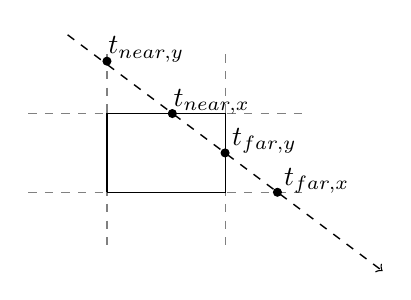
\begin{tikzpicture}[y=0.5cm, x=.5cm,font=\sffamily]
      % Planes
      \draw[dashed, color=gray] (-2,0) -- (5,0);
      \draw[dashed, color=gray] (-2,2) -- (5,2);
      \draw[dashed, color=gray] (0,3.5) -- (0,-1.5);
      \draw[dashed, color=gray] (3,3.5) -- (3,-1.5);

      % AABB
      \draw (0,0) -- (3,0) -- (3,2) -- (0,2) -- (0,0);

      % Ray
      \drawRay{-1,4}{7,-2}

      % Intersection
      \draw[fill=black] (0,3.33) circle (0.05cm);
      \draw (1,3.63) node{$t_{near,y}$};
      \draw[fill=black] (1.66,2) circle (0.05cm);
      \draw (2.66,2.3) node{$t_{near,x}$};
      \draw[fill=black] (3,1) circle (0.05cm);
      \draw (4,1.3) node{$t_{far,y}$};
      \draw[fill=black] (4.33,0) circle (0.05cm);
      \draw (5.33,0.3) node{$t_{far,x}$};

    \end{tikzpicture}
  }
  \caption{Ray/Box intersection.}
  \label{fig:rayBoxIntersection}
\end{figure}

Clearly kd-trees provide the simplest distance calculations of the
above given examples.

% Example of kd-tree flexibility over octree (important in sparse
% scenes / empty space partitioning)

Binary trees, such as kd- and bsp trees, are also more flexible than
\textit{quadtress} or \textit{octrees}, which subdivides the geometry
with 2 or 3 planes respectively per node. An example can be seen on
\reffig{fig:binQuadSplit}. This flexibility can be extremely important
when accelerating sparse scenes.

\fixme{include trees in the bsp/quad figure}

\begin{figure}
  \centering
  \subfloat[Possible binary splits.]{
    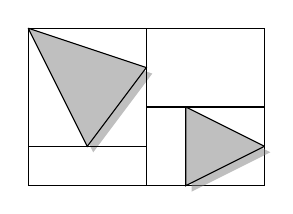
\begin{tikzpicture}[y=0.5cm, x=.5cm,font=\sffamily]
      
      % AABB
      \draw (0,0) -- (6,0) -- (6,4) -- (0,4) -- (0,0);
      
      % TRIS
      \drawTri{0,4}{3,3}{1.5,1}
      \drawTri{6,1}{4, 2}{4,0}
      
      % splits
      \draw (3,0) -- (3,4);
      \draw (0,1) -- (3,1);
      \draw (3,2) -- (6,2);
      
    \end{tikzpicture}
    \label{fig:binarySplit}
  }
  \hspace{20pt}
  \subfloat[Possible quadternary splits.]{
    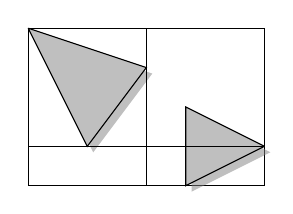
\begin{tikzpicture}[y=0.5cm, x=.5cm,font=\sffamily]
      
      % AABB
      \draw (0,0) -- (6,0) -- (6,4) -- (0,4) -- (0,0);
      
      % TRIS
      \drawTri{0,4}{3,3}{1.5,1}
      \drawTri{6,1}{4, 2}{4,0}
      
      % splits
      \draw (3,0) -- (3,4);
      \draw (0,1) -- (6,1);
      
    \end{tikzpicture}
    \label{fig:quadternarySplit}
  }

  \parbox{9cm}{\caption[Comparisson of binary and quadternary
      splitting]{A comparisson of binary and quadternary
      splitting. Notice that the binary splitting planes can be placed
      without intersecting any geometry.}\label{fig:binQuadSplit}}
\end{figure}

% Vlastimil Havran did an extensive study of available spatial
% subdivision schemes (including regular grids, nested grids, octrees
% and kd-trees) and concludes in his phd thesis that kd-trees are
% better than the other schemes in most cases.

Finally, in his phd. dissertation, Vlastimil Havran did an extensive
study of spatial data structures, including grids, octress and
kd-trees, and found that the kd-tree performed the best in most cases.

Given all of the above and with the recent paper by \zhou{}, in which
kd-trees are constructed in real-time on graphics hardware, it is easy
to see why the choice fell on kd-trees as the acceleration structure.

% About this Chapter. Start by motivation. Then explain how kd-trees
% are constructed, including different strategies for choosing the
% spliting plane and doing the actual geometry splitting. Then the
% chapter will end with a discussion of how to implement the
% algorithms efficiently on a SIMT architecture.

In the rest of this chapter, we will first examine how kd-trees are
built. In particular different algorithms for choosing the splitting
plane candidate will be studied and how to handle geometry
intersecting the splitting plane will be discussed. The latter part of
this chapter deals with converting a sequential kd-tree construction
algorithm into a dataparallel algorithm. Focus is split between upper
tree nodes and lower tree nodes, once the number of geometric
primitives per node goes below a certain threshold.

\section{Building KD-trees}

A kd-tree is a binary tree that recursively subdivides geometry into
smaller tree nodes. \refalg{alg:kdTreeCreator} describes a generel
recursive kd-tree construction scheme.

\begin{algorithm}
  \caption{Recursive kd-tree constructor}
  \label{alg:kdTreeCreator}
  \begin{algorithmic}
    \PROCEDURE{ConstructKDTree}
              {$T$ : Triangle List; $voxel$ : AABB}
              {$node$ : KDNode}
              {\IF{IsLeaf($T, voxel$)}
                  \ASSIGN{$node$}{Leaf(T)}
                \ELSE
                  \COMMENTIT{Determining the splitting plane will be discussed in \refsection{sec:splittingPlane}}
                  \ASSIGN{$plane$}{DeterminePlane($T, voxel$)}
                  \ASSIGN{$(voxel_L, voxel_R)$}{Split($voxel, p$)}
                  \COMMENTIT{How to associate geometry with a voxel will be the topic of  \refsection{sec:splittingGeom}}
                  \ASSIGN{$T_L$}{AssociateGeometry($T, voxel_L$)}
                  \ASSIGN{$T_R$}{AssociateGeometry($T, voxel_R$)}
                  \ASSIGN{$node$}{Node($plane$, ConstructKDTree($T_L, voxel_L$), ConstructKDTree($T_R, voxel_R$))}
                \ENDIF}
  \end{algorithmic}
\end{algorithm}

ConstructKDTree takes as arguments a list of triangles and an axis
aligned bounding box defining the volume of the node. The algorithm
then checks if the triangles and bounding box satisfy the requirements
of being a leaf node. If so, then a leaf is produced and the recursion
terminates. If not, then a splitting plane, $plane$, needs to be
determined and the bounding box is divided by $plane$, producing a new
left and right axis aligned bounding box. Triangles are then
distributed to each new bounding box by an association algorithm and a
new node is created that will contain references to it's 2
children. An example of an iteration of ConstructKDTree can be seen in
\reffig{fig:kdIteration}.

\begin{figure}
  \centering \subfloat[A simple scene and it's corrosponding
    kd-tree. The entire scene is contained in the root node.]{
    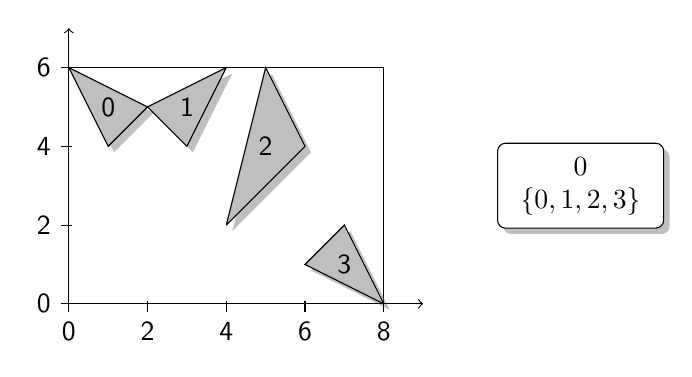
\begin{tikzpicture}[y=0.5cm, x=0.5cm,font=\sffamily]
      \drawNode{0,0}{8,0}{8,6}{0,6}
      
      % Tris
      \drawTri{0,6}{1,4}{2,5}
      \draw (1,5) node{0};
      \drawTri{4,6}{3,4}{2,5}
      \draw (3,5) node{1};
      \drawTri{4,2}{5,6}{6,4}
      \draw (5,4) node{2};
      \drawTri{8,0}{7,2}{6,1}
      \draw (7,1) node{3};

      %axes
      \draw[->] (0,0) -- coordinate (x axis mid) (9,0);
      \draw[->] (0,0) -- coordinate (y axis mid) (0,7);
      %ticks
      \foreach \x in {0,2,...,9}
     		\draw (\x,1pt) -- (\x,-3pt)
			node[anchor=north] {\x};
    	\foreach \y in {0,2,...,7}
     		\draw (1pt,\y) -- (-3pt,\y) 
     			node[anchor=east] {\y}; 

      \draw (13,3) node [leaf] (0){$\begin{array}{c}0\\\{0, 1, 2, 3\}\end{array}$};
    \end{tikzpicture}
    \label{fig:simpleScene0}
  }

  \subfloat[The same scene as in \reffig{fig:simpleScene0}. The
    kd-tree has split the geometry down the middle and created 2 new
    leaf nodes. The geometry has then been associated with these 2
    leaf nodes.]{
    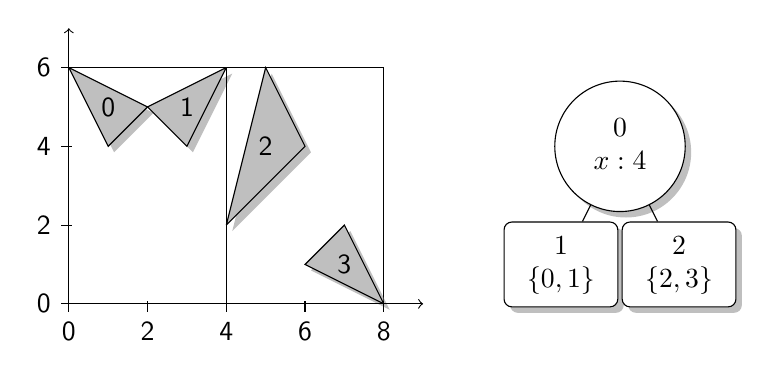
\begin{tikzpicture}[y=0.5cm, x=0.5cm,font=\sffamily]
      \drawNode{0,0}{8,0}{8,6}{0,6}
      
      % Tris
      \drawTri{0,6}{1,4}{2,5}
      \draw (1,5) node{0};
      \drawTri{4,6}{3,4}{2,5}
      \draw (3,5) node{1};
      \drawTri{4,2}{5,6}{6,4}
    \draw (5,4) node{2};
      \drawTri{8,0}{7,2}{6,1}
      \draw (7,1) node{3};

      % Splits
      \draw (4,0) -- (4,6);

      %axes
      \draw[->] (0,0) -- coordinate (x axis mid) (9,0);
      \draw[->] (0,0) -- coordinate (y axis mid) (0,7);
      %ticks
      \foreach \x in {0,2,...,9}
     		\draw (\x,1pt) -- (\x,-3pt)
			node[anchor=north] {\x};
      \foreach \y in {0,2,...,7}
     		\draw (1pt,\y) -- (-3pt,\y) 
     			node[anchor=east] {\y}; 

      \draw (14,4) node [node] (0){$\begin{array}{c}0\\x:4\end{array}$}
        child {node [leaf] (1) {$\begin{array}{c}1\\\{0, 1\}\end{array}$}}
        child {node [leaf] (2) {$\begin{array}{c}2\\\{2, 3\}\end{array}$}};
    \end{tikzpicture}
  }
  \caption{One iteration of the kd-tree construction algorithm.}
  \label{fig:kdIteration}
\end{figure}

% Left balanced non pointer vs pointers

In generel there are 2 ways a node can reference its child nodes. The
first is \textit{balanced trees}, where children of a node can be
addressed implicitly without the use of pointers. The reason for this
is that nodes at the same tree level are placed sequantially in
memory. The left and right child of node $n$ can then be indexed using
$2n+1$ and $2n+2$. The parent of a node is indexed with $\lceil n/2
\rceil - 1$.

% Balanced trees suck, example of partition with high density in one
% side and no triangles in other side. 

Wald et al.\citebook{wald:04:VVH} has the following to say about
balanced trees.

\quotebook{Balancing is optimal only for binary searching, and if all
  nodes have equal access probabilities. Neither of these two
  prerequisites are fulfilled for range queries (such as ray traversal
  and kNN queries), nor for unevenly distributed primitives such as
  photons or triangles.}{wald:04:VVH}

% Choose pointers as that would lead to less memory consumption and it
% places all nodes of the same level in a continues block, making it
% easier to work with them.

To avoid balanced trees we can instead use pointers to reference the
children. This allows for more flexibility when creating the tree.
Unfortunatly it also means storing more data per node and in the case
of slow memory access it could cause a memory latency
bottleneck. However, when experimenting with different techniques such
as is done in this thesis, the added flexibility can be a benefit and
in \refsection{sec:gpuEmptySpace} we shall see how this flexibility
can be used to add empty space maximizing, something that could not
have been done as unobtrusive had the tree been balanced.

% Triangle references

A kd-tree leaf node must be able to reference the triangles associated
with it. In this thesis I have choosen the convention that triangles
associated with a node must be placed sequentially in memory and
therefore a leaf need only contain the index of its first triangle and
the amount of triangles it is associated with.

\subsection{Choosing the Splitting Plane}\label{sec:splittingPlane}

\fixme{does this section describe clipping well enough? That false
  primitives can accumulate over successive splits?}

% All the brilliance in KD-tree construction comes down to choosing
% the splitting plane and deciding when to stop.

Looking again at \refalg{alg:kdTreeCreator}, we can see that all the
brilliance in constructing a high quality kd-tree is knowing where to
place the splitting plane and when to end the recursion and create a
leaf.

% Different splitting planes heuristics.

In the following section 2 algorithms that solves this problem is
presented and then extended with empty space maximizing.


\subsubsection{Spatial Median}

% Split at the spatial median.

% Axis to split along can be choosen in a round robin fashion or the
% largest axis can be choosen. (Which initially minimises the surface
% of the children)

A quite simple method of choosing the splitting plane is to place it
at the spatial median of the nodes bounding box. There are 2 ways to
choose which dimensional spatial median to use. A \textit{round robin}
fashion can be used, where the dimensions are cycled every iteration;
ie. when creating the first node the plane will lie perpendicular to
the x-axis, the children will then be split along the y-axis, in the
next iteration the plane will split along the z-axis and then restart
again at x. Another way of choosing the dimension is to split along
the largest axis of the node's bounding box. This can be more costly
than the round robin approach, since the entire bounding box will have
to be calculated each iteration, but it will also produce the best
results.

The termination requirement for spatial median splitting is equally as
simple as choosing the splitting plane. If the number of triangles per
node falls below a certain threshold, iteration stops.

% Refered to as the naïve implementation in Wald07.

This method is refered to as naïve in \citebook{wald:06:NlogN} and
rightly so. Not much thought is put into the distribution of geometry
inside the bounding box. On \reffig{fig:crapMedian} an example is
given where the node is split in a non-intuitive way. Spatial median
splitting does, however, make up for its suboptimal splitting planes
by being quite fast, and I will therefore use it for creating my
kd-trees upper nodes, as is described in \refsection{sec:upperNodes}.

\begin{figure}
  \centering
  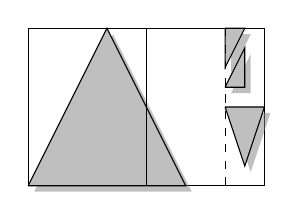
\begin{tikzpicture}[y=0.5cm, x=.5cm,font=\sffamily]
    % AABB
    \draw (0,0) -- (6,0) -- (6,4) -- (0,4) -- (0,0);

    % Tris
    \drawTri{0,0}{2,4}{4,0}
    \drawTri{5,4}{5.5,4}{5,3}
    \drawTri{5,2.5}{5.5,2.5}{5.5,3.5}
    \drawTri{5,2}{6,2}{5.5,0.5}

    % Split
    \draw (3,0) -- (3,4);
    \draw[dashed] (5,0) -- (5,4);

  \end{tikzpicture}

  \vspace{3mm}
  \parbox{5cm}{\caption[A poor split produced by median splitting.]{A
      poor split produced by median splitting. The solid line is a
      median split. The dashed one is a more optimal splitting plane,
      since it divides the large triangle from the
      small.}\label{fig:crapMedian}}
\end{figure}

\subsubsection{Surface Area Heuristic}

% SAH assumptions can be seen in Wald07

A far better splitting plane position can be obtained by applying the
\textit{surface area heuristic}, \textit{SAH}. Instead of only
considering the bounding volume surrounding the geometry, SAH
considers the entire geometry of a node. In essence SAH computes the
\textit{expected cost} of traversing a node, $N$, with child nodes $L$
and $R$.

\begin{displaymath}
  SAH(N \rightarrow \{L, R\}) = C_N + \frac{C_L A_L}{A_N} +
  \frac{C_R A_R}{A_N}
\end{displaymath}

where $C_N$ is the cost of traversing the node itself and is
independent of the splitting plane, $C_L$ is the cost of traversing
the left child node and $C_R$ is the cost of traversing the right
child node. $A_n$ is the summed surface area of all primitives in node
$n$. Choosing the best splitting plane amounts to applying SAH to all
possible splitting planes and then choosing the one with lowest
cost. Since the above cost evaluation does not take rays into account,
SAH assumes that rays are uniformly distributed, infinite lines.

SAH can also automatically determine when to stop splitting. Assuming
that the cost of intersecting a leaf is given as $C_{leaf} = \|T\| *
C_i$, where $\|T\|$ is the number of triangles and $C_i$ is the cost of
intersecting a triangle. SAH's termination criteria is then $C_{leaf}
< C_N$, i.e. SAH terminates when the cost of intersecting a leaf
becomes less than the cost of most optimal splitting plane.

% Globlly optimal is infeasable for complex scenes and instead a local
% greedy approximation is used.

Calculating a globally optimal solution using SAH is infeasable,
except for trivially simple scenes. A \textit{local greedy
  approximation} is used instead, where it is assumed that the created
child nodes are leafs. The makes the costs $C_L$ and $C_R$ equal to
the amount of primitives contained in the left and right child node.

Inspite of all the assumptions made by SAH, which in practice do not
hold, it is still considered one of the best heuristics and produces
trees of the highest quality.

% SAH calculation optimizations include axis round robin and some damn
% paper I can't remember.


\paragraph{Split Candidates}

% To avoid having to test the infinitely many splitting planes
% possible, we instead have to choose sensible planes for SAH.

As mentioned above the SAH cost needs to be calculated for
\textit{all} available splitting planes. Since there infinitely many
potential planes along either axis, we need some method to distinguish
useful split candidates from unimportant ones. That means we're only
interested in those finitely many planes where the geometry
association in the resulting left and right child nodes change.

% Take planes from bounding volumes

The obvious choice is to use the 6 planes defined by the triangles
axis aligned bounding box. While this is a simple and fast solution,
it can create a bloated tree, since triangles do not necessarily
overlap a node's bounding box, simply because its own bounding box
does. An example can be seen on \reffig{fig:aabbSplit}

\begin{figure}
  \centering
  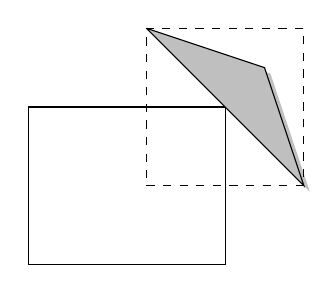
\begin{tikzpicture}[y=0.5cm, x=.5cm,font=\sffamily]

    % AABB
    \draw (0,0) -- (5,0) -- (5,4) -- (0,4) -- (0,0);

    \drawTri{3,6}{7,2}{6,5}
    \drawAabb{3,2}{7,2}{7,6}{3,6}

  \end{tikzpicture}

  \vspace{3mm}
  \parbox{5cm}{\caption[Triangle/Node bounding box intersection.]{An
      example of how a triangles bounding box, the dashed box, can
      overlap a nodes bounding box, while the triangle itself does
      not.}\label{fig:aabbSplit}}
\end{figure}

Another problem with this approach is that bounding boxes of small
nodes may be completely contained inside the geometry's bounding box
and thus none of the planes are actually useful split
candidates. \reffig{fig:aabbContained} demonstrates this.

\begin{figure}
  \centering
  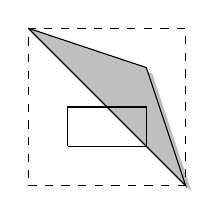
\begin{tikzpicture}[y=0.5cm, x=.5cm,font=\sffamily]

    \drawTri{0,4}{4,0}{3,3}
    \drawAabb{0,0}{4,0}{4,4}{0,4}

    % AABB
    \draw (1,1) -- (3,1) -- (3,2) -- (1,2) -- (1,1);

  \end{tikzpicture}
    
  \vspace{3mm}
  \parbox{5cm}{\caption[A tree node's bounding box contained in a
      triangle's bounding box.]{The kd-tree node's bounding box
      completely contained inside the triangles bounding
      box.}\label{fig:aabbContained}}
\end{figure}

A solution is to continuously \textit{clip} the bounding box of the
split geometry to fit the part of the geometry inside the tree nodes
bounding box, creating \textit{perfect split} condidates, as
demonstrated on \reffig{fig:aabbClipped}.

\begin{figure}
  \centering
  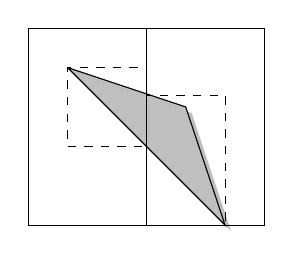
\begin{tikzpicture}[y=0.5cm, x=.5cm,font=\sffamily]

    \drawTri{0,4}{4,0}{3,3}
    \drawAabb{0,2}{2,2}{2,4}{0,4}
    \drawAabb{2,0}{4,0}{4,3.3}{2,3.3}

    % AABB
    \drawNode{-1,0}{2,0}{2,5}{-1,5}
    \drawNode{2,0}{5,0}{5,5}{2,5}

  \end{tikzpicture}

  \vspace{3mm}
  \parbox{5cm}{ \caption[Triangle clipping.]{The triangles bounding
      box has been clipped to fit the part of the triangle contained
      in the nodes bounding boxes.}\label{fig:aabbClipped}}
\end{figure}

Another solution is to simply remove the offending triangles, reafter
refered to as \textit{false primitives}, from the node. This can be
done by performing a triangle/box intersection check, a derivation of
the \textit{seperating axis theorem}, as described by Möller in
\citebook{Moller:2005}.


\subsubsection{Empty Space Maximizing}\label{sec:emptySpace}

An effective optimization to the quality of kd-trees is \textit{empty
  space maximization}. The idea behind the optimization is to cut away
large empty parts of the scene. This is done by placing empty leaf
nodes in the upper parts of the tree. The empty nodes will provide rays
traversing the tree with an early out option, skipping a large portion
of the geometry. 

\reffig{fig:noEmptySpaceExample} shows a simple scene without empty
space cut away and its corrosponding kd-tree. Without empty space
maximization the ray entering the scene from the lower left cornor is
forced to perform intersection test with every triangle in leaf node
1. In contrast the kd-tree in\reffig{fig:emptySpaceExample} has been
created with empty space maximization enabled and the ray entering the
scene now ends up in leaf 4. Leaf 4 is empty and allows the ray to
advance forward while skipping every triangle in leaf 1.

\begin{figure}
  \centering
  \subfloat[A simple scene without empty space cut away.]{
    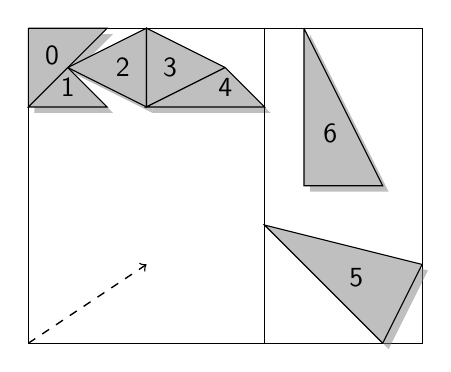
\begin{tikzpicture}[y=0.5cm, x=.5cm,font=\sffamily]
      
      % AABB
      \draw (0,0) -- (10,0) -- (10,8) -- (0,8) -- (0,0);
      
      % Tris
      \drawTri{9,0}{10,2}{6,3}
      \draw (8.33,1.66) node {5};
      \drawTri{7,8}{7,4}{9,4}
      \draw (7.67,5.33) node {6};
      
      \drawTri{0,8}{0,6}{2,8}
      \draw (0.6,7.3) node {0};
      \drawTri{1,7}{0,6}{2,6}
      \draw (1,6.5) node {1};
      \drawTri{1,7}{3,6}{3,8}
      \draw (2.4,7) node {2};
      \drawTri{5,7}{3,6}{3,8}
      \draw (3.6,7) node {3};
      \drawTri{5,7}{3,6}{6,6}
      \draw (5,6.5) node {4};
      
      % Splits
      \draw (6,0) -- (6,8);
      
      % Ray
      \drawRay{0,0}{3,2}
      
    \end{tikzpicture}
    \label{fig:noEmptySpaceScene}
  }
  \hspace{5mm}
  \subfloat[The tree corrosponding to the scene in \reffig{fig:noEmptySpaceScene}.]{
    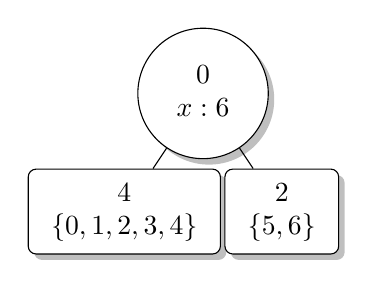
\begin{tikzpicture}[y=0.5cm, x=.5cm,font=\sffamily,
        level/.style={sibling distance=20mm/#1}]
      \node [node] {$\begin{array}{c}0\\x:6\end{array}$}
        child {node [leaf] {$\begin{array}{c}4\\\{0,1,2,3,4\}\end{array}$}}
        child {node [leaf] {$\begin{array}{c}2\\\{5, 6\}\end{array}$}};
    \end{tikzpicture}
    \label{fig:noEmptySpaceTree}
  }
  
  \caption[Scene without empty space maximization.]{A kd-tree
    constructed around a simple scene. The kd-tree doesn't use the
    empty space maximization optimization.}
  \label{fig:noEmptySpaceExample}
\end{figure}

\begin{figure}
  \centering
  \subfloat[The scene from \reffig{fig:noEmptySpaceScene} with empty space cut away.]{
    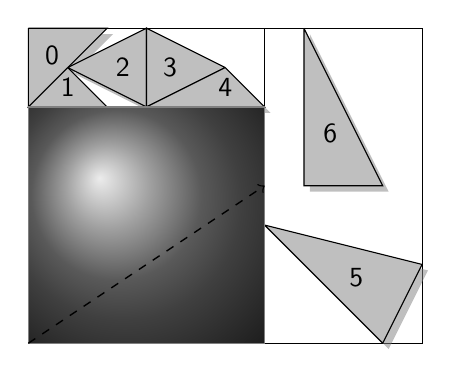
\begin{tikzpicture}[y=0.5cm, x=.5cm,font=\sffamily]
      
      % AABB
      \draw (0,0) -- (10,0) -- (10,8) -- (0,8) -- (0,0);
      
      % Tris
      \drawTri{9,0}{10,2}{6,3}
      \draw (8.33,1.66) node {5};
      \drawTri{7,8}{7,4}{9,4}
      \draw (7.67,5.33) node {6};
      
      \drawTri{0,8}{0,6}{2,8}
      \draw (0.6,7.3) node {0};
      \drawTri{1,7}{0,6}{2,6}
      \draw (1,6.5) node {1};
      \drawTri{1,7}{3,6}{3,8}
      \draw (2.4,7) node {2};
      \drawTri{5,7}{3,6}{3,8}
      \draw (3.6,7) node {3};
      \drawTri{5,7}{3,6}{6,6}
      \draw (5,6.5) node {4};
      
      % Splits
      \draw (6,0) -- (6,8);
      \draw (0,6) -- (6,6);
      
      % Empty space
      \draw[ball color=gray, color=green, shading=ball,gray] (0,0) -- (0,6) -- (6,6) -- (6,0) -- (0,0);
      
      % Ray
      \drawRay{0,0}{6,4}
      
    \end{tikzpicture}
    \label{fig:emptySpaceScene}
  }
  \hspace{5mm}
  \subfloat[The tree from \reffig{fig:noEmptySpaceTree} with the empty space nodes 3 and 4 injected.]{
    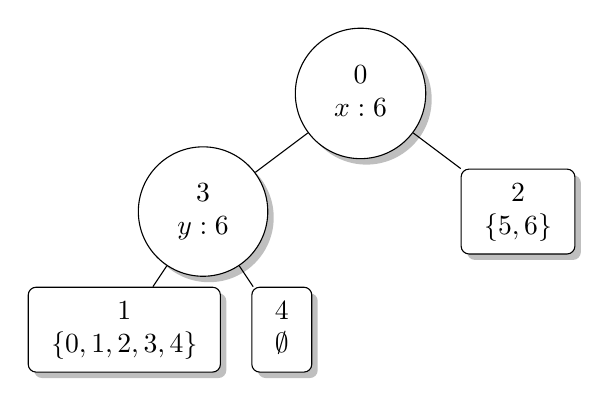
\begin{tikzpicture}[y=0.5cm, x=.5cm,font=\sffamily,
        level/.style={sibling distance=40mm/#1}]
      \node [node] {$\begin{array}{c}0\\x:6\end{array}$}
        child {node [node] {$\begin{array}{c}3\\y:6\end{array}$}
            child {node [leaf] {$\begin{array}{c}1\\\{0,1,2,3,4\}\end{array}$}}
            child {node [leaf] {$\begin{array}{c}4\\\emptyset\end{array}$}}
        }
        child {node [leaf] {$\begin{array}{c}2\\\{5, 6\}\end{array}$}};
    \end{tikzpicture}
    \label{fig:emptySpaceTree}
  }
  
  \caption[Empty space maximization.]{An example of empty space
    maximizing. The grey ball shaded area represents an empty node and
    allows the ray to leap across it and skip intersection tests with
    the 5 triangles above.}\label{fig:emptySpaceExample}
\end{figure}


Unfortunatly, how large a percentage of a node that should be empty
before empty space splitting can cut it away is highly scene specific,
making this optimization less usefull in the general case. Like \zhou{}
I have found that performing an empty space split is optimal when a
bounding box is more than 25\% empty along one of the axes.

% Dynamic empty space threshold, favor early out in the top of the tree.

% huge ray tracing performance improvement in testscene (23% without
% raytracers doing intersection tests at leaf nodes)

% Implementation is 

\subsection{Triangle/Node Association Schemes}\label{sec:splittingSchemes}

When a splitting plane has been chosen, the triangles in the split
kd-tree node needs to be associated with the two newly created leaf
nodes that they overlap. Triangles located entirely in front of the
splitting plane are associated with the left child node and triangles
entirely behind are associated with the right child node. The
association schemes discussed in this section present different
methods for handling the triangles intersected by the splitting
plane. The scheme employed is important in dynamic schemes. On one
hand a fast approximating association scheme may assign triangles to
nodes that do not necessarily contain them, resulting in larger trees
and slower ray tracing times. On the other hand a scheme rigorously
checking every triangle and only assigning triangles to nodes that
they definetly intersect will result in a smaller tree and faster ray
tracing time, but results in more time being spend creating the
acceleration structure.


%% This section will look at alternatives to triangle splitting, namely
%% \textit{triangle division}, where the triangle is not split by
%% splitting planes, but divided onto each side, by simply adjusting it's
%% bounding box, and \textit{box inclusion}, where the triangles
%% themselves are not tested for inclusion, but their bounding boxes are.

% What to do with the triangles caught in the splitting plane.


\subsubsection{Triangle splitting}

% Normally ppl split.

The most common approach when a triangle should be divided around a
splitting plane, is to actually split the triangle up into new
triangles. New triangles produced by triangle splitting will always be
located entirely within the bounding box of the kd-node they are
associated with. When performing triangle splitting there are 3 cases
to look out for, as can be seen in \reffig{fig:splittingCases}.

\begin{figure}
  \centering
  \subfloat[2 vertices to the left of the splitting plane.]{
    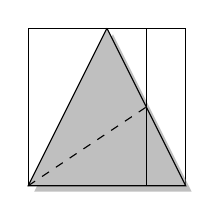
\begin{tikzpicture}[y=0.5cm, x=.5cm,font=\sffamily]
      \draw (0,0) -- (4,0) -- (4,4) -- (0,4) -- (0,0);
      \drawTri{2,4}{0,0}{4,0}
      \draw[dashed] (0,0) -- (3,2);
      \draw (3,0) -- (3,4);
    \end{tikzpicture}
    \label{fig:splittingCase1}
  }
  \hspace{5mm}
  \subfloat[1 vertex intersected by the splitting plane.]{
    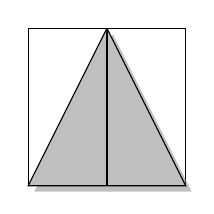
\begin{tikzpicture}[y=0.5cm, x=.5cm,font=\sffamily]
      \draw (0,0) -- (4,0) -- (4,4) -- (0,4) -- (0,0);
      \drawTri{2,4}{0,0}{4,0}
      \draw (2,0) -- (2,4);
    \end{tikzpicture}
    \label{fig:splittingCase2}
  }
  \hspace{5mm}
  \subfloat[2 vertices to the right of the splitting plane.]{
    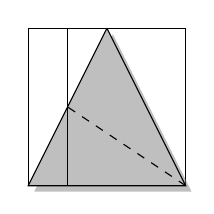
\begin{tikzpicture}[y=0.5cm, x=.5cm,font=\sffamily]
      \draw (0,0) -- (4,0) -- (4,4) -- (0,4) -- (0,0);
      \drawTri{2,4}{0,0}{4,0}
      \draw[dashed] (4,0) -- (1,2);
      \draw (1,0) -- (1,4);
    \end{tikzpicture}
    \label{fig:splittingCase3}
  }

  \vspace{3mm}
  \parbox{10cm}{\caption{The 3 different triangle splitting cases. A dashed line
      represents an additional split needed to keep representing
      geometry as triangles.}\label{fig:splittingCases}}
\end{figure}

The first case in \reffig{fig:splittingCase1} illustrates the split
when 2 vertices are located on the left of the splitting plane and one
on the right. This case is mirrored by \reffig{fig:splittingCase3}
where 2 of the vertices are located to the right of the splitting
plane. In both of these cases a triangle split will produce three new
triangles. In the last case in \reffig{fig:splittingCase2} one of the
vertices is directly intersected by the splitting plane and splits the
triangle perfectly into two new triangles. This last case however is
highly unlikely and in generel a triangle split always produces 3 new
triangles. 


\subsubsection{Triangle dividing}

\begin{figure}
  \centering
  \subfloat[One split.]{
    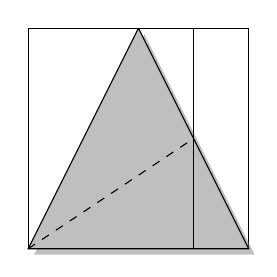
\begin{tikzpicture}[y=0.7cm, x=0.7cm,font=\sffamily]
      \draw (0,0) -- (4,0) -- (4,4) -- (0,4) -- (0,0);
      \drawTri{2,4}{0,0}{4,0}
      \draw[dashed] (0,0) -- (3,2);
      \draw (3,0) -- (3,4);
    \end{tikzpicture}
  }
  \subfloat[Two splits.]{
    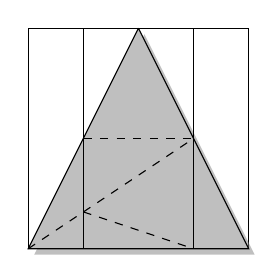
\begin{tikzpicture}[y=0.7cm, x=0.7cm,font=\sffamily]
      \draw (0,0) -- (4,0) -- (4,4) -- (0,4) -- (0,0);

      \drawTri{2,4}{0,0}{4,0}
      
      \draw (1,0) -- (1,4);
      \draw (3,0) -- (3,4);

      \draw[dashed] (1,2) -- (3,2);
      \draw[dashed] (0,0) -- (3,2);
      \draw[dashed] (1,0.667) -- (3,0);
    \end{tikzpicture}
  }
  \subfloat[Three splits.]{
    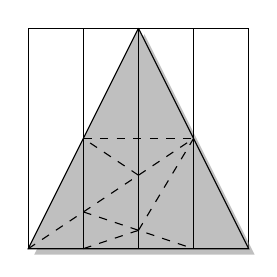
\begin{tikzpicture}[y=0.7cm, x=0.7cm,font=\sffamily]
      \draw (0,0) -- (4,0) -- (4,4) -- (0,4) -- (0,0);
      \drawTri{2,4}{0,0}{4,0}
      
      \draw (1,0) -- (1,4);
      \draw (2,0) -- (2,4);
      \draw (3,0) -- (3,4);

      \draw[dashed] (1,2) -- (3,2);
      \draw[dashed] (0,0) -- (3,2);
      \draw[dashed] (1,0.667) -- (3,0);
      \draw[dashed] (2,0.333) -- (1,0);
      \draw[dashed] (2,0.333) -- (3,2);
      \draw[dashed] (2,1.333) -- (1,2);
    \end{tikzpicture}
  }
  \caption[Excessive splitting of a triangle.]{The triangle splitting
    algorithm performing excessive splits on a triangle.}
  \label{fig:excessiveSplitting}
\end{figure}

Splitting a triangle almost always produce 3 triangles and can lead to
excessively many new triangles being created, as evidenced by
\reffig{fig:excessiveSplitting}. The problem with excessive splitting
is that each new triangle actually represents the original triangle
and so on \reffig{fig:excessiveSplitting} we see nodes containing up
to 6 triangles, all representing the exact same original and
cluttering up the tree with unnecessary geometry. A more preferable
situation is seen in \reffig{fig:dividing}, where each node only
contains one reference to the original triangle.

\begin{figure}
  \centering
  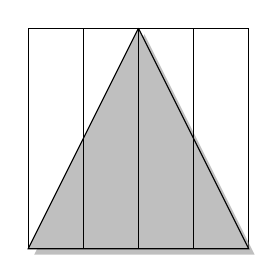
\begin{tikzpicture}[y=0.7cm, x=0.7cm,font=\sffamily]
    \draw (0,0) -- (4,0) -- (4,4) -- (0,4) -- (0,0);
    \drawTri{2,4}{0,0}{4,0}
    
    \draw (1,0) -- (1,4);
    \draw (2,0) -- (2,4);
    \draw (3,0) -- (3,4);
  \end{tikzpicture}
  
  \vspace{3mm}
  \parbox{5cm}{\caption[Dividing a triangle.]{Dividing a triangle
      among the nodes owning it. Notice that each node only contains
      one reference to the original triangle.}\label{fig:dividing}}
\end{figure}

This is the central idea behind \textit{dividing triangles}. Instead
of splitting a triangle around the splitting plane and creating new
triangles, I associated the original triangle with the new
nodes. Wether or not to associate a triangle and node is decided by
performing a \textit{triangle/bounding box overlap} test, as described
in Möller\citebook{Moller:2005}. If the triangle overlaps the child
node's bounding box after the split, then it will be associated with
that node, otherwise the triangle is excluded from the node.


\subsubsection{Box Inclusion}

% Simpler than splitting.

Performing the triangle/bounding box overlap test can be a
computationally heavy task. A cheaper splitting scheme is to test a
triangle's axis aligned bounding volume with the axis aligned bounding
volume of the node. Given that an axis aligned bounding volume, $v$,
can be described by its minimum and maximum value along each axis, I
define it as $v = \{v_{min}, v_{max}\} \in \{R^3, R^3\} $. Performing
the intersection test between the triangle's bounding volume, $t$, and
the node's, $n$, then becomes $n_{min} < v_{max} \wedge v_{min} <
n_{max}$.

\begin{figure}
  \centering
  \subfloat[]{
    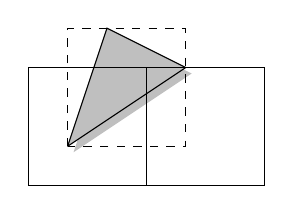
\begin{tikzpicture}[y=0.5cm, x=.5cm] 
      \drawTri{1,1}{2,4}{4,3}
      \drawAabb{1,1}{1,4}{4,4}{4,1}
      
      \draw (0,0) -- (0,3) -- (3,3) -- (3,0) -- (0,0);
      \draw (3,0) -- (3,3) -- (6,3) -- (6,0) -- (3,0);
    \end{tikzpicture}
  }
  \subfloat[hut]{
    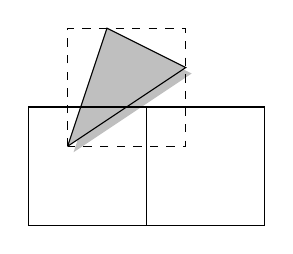
\begin{tikzpicture}[y=0.5cm, x=.5cm]
      \drawTri{1,2}{2,5}{4,4}
      \drawAabb{1,2}{1,5}{4,5}{4,2}

      \draw (0,0) -- (0,3) -- (3,3) -- (3,0) -- (0,0);
      \draw (3,0) -- (3,3) -- (6,3) -- (6,0) -- (3,0);
    \end{tikzpicture}
    \label{fig:falseBoxInclusion}
  }
  \caption{Box inclusion examples.}
  \label{fig:boxInclusion}
\end{figure}

% Naturally increases amount of \textit{false primitives} in the tree, but is
% very cheap.

\refFig{fig:boxInclusion} shows two examples of a node being split
down the middle. In both examples the triangle will be associated with
both new nodes, as the triangles bounding box overlaps both nodes. But
in \reffig{fig:falseBoxInclusion} we clearly see that the triangle
itself does not overlap the right node's bounding box. This
illustrates the drawback to only testing a triangle's bounding box and
how box inclusion will produce false positives. Triangles that do not
intersect a nodes bounding box can be associated with that node and
become a false primitive, which will increase the size of the tree and
slow down ray tracing time. However, box inclusion makes up for this
by performing fast node/triangle association, cutting down on the time
spend constructing the tree.

% Also has an increased change of looping during construction in
% combination with a small max lower size. Fx fairy forest loops using
% adjusting bounding box with a max size of 32 primtives in leaf nodes.

% False primitives can then be removed at a later stage at the cost of
% some extra overhead. Or combine with Divide every n'th step for
% optimal sweetness.

% With the added leaf intersection in the raytracer, extra triangles
% in the leaf nodes become even less important and this method starts
% to shine for dynamic scenes.






\section{Adopting the Algorithms for CUDA}

% Needs to exploit the dataparallel nature of GPU's A GPU needs as
% many of its multiprocessors occupied as possibly for optimal
% performance.

Having explored the different methods for deciding which splitting
plane to use and how to associate geometry with a node in the kd-tree,
it is time to look at the actual implementation of a kd-tree
construction algorithm on the GPU.

The generel kd-tree construction method presented in
\refalg{alg:kdTreeCreator} recursively constructs \textit{one} tree
node at a time in a \textit{depth-first} manor. In order to
efficiently utilize the GPU, as many of it's multiprocessors as
possible must be fully occupied. This means \refalg{alg:kdTreeCreator}
must be restructured to work on multiple nodes at a time. Fortunatly
this is exactly what \zhou{} did by changing the kd-tree constructor
to work on a list of nodes and recursively create the tree in
\textit{breadth-first} order, as outlines in
\refalg{alg:bfsKDTreeCreator}.

\begin{algorithm}
  \caption{BFS Recursive kd-tree constructor}
  \label{alg:bfsKDTreeCreator}
  \begin{algorithmic}
    \PROCEDURE{ConstructKDTree}
              {$activeNodes$ : Node List  \textit{\color{gray}//list of kd-nodes not processed yet}}
              {$nextNodes$ : Node List}
              {\PARALLELFOR{$node$}{$activeNodes$}
                 \IF{IsLeaf($node$)}
                   \ASSIGN{$node$}{Leaf($node$)}
                 \ELSE
                   \COMMENTIT{Determine the splitting plane.}
                   \ASSIGN{$plane$}{DeterminePlane($node$)}
                   \ASSIGN{$(node_L, node_R)$}{Split($node, p$)}
                   \COMMENTIT{Associate the geometry with a node and add it to the next list.}
                   \ASSIGN{$node_L.geometry$}{AssociateGeometry($node.geometry, node_L$)}
                   \STATE{$nextNodes$.Add($node_L$)}
                   \ASSIGN{$node_R.geometry$}{AssociateGeometry($node.geometry, node_R$)}
                   \STATE{$nextNodes$.Add($node_R$)}
                 \ENDIF
               \ENDFOR}
  \end{algorithmic}
\end{algorithm}

% Creating the KD-tree in BFS will optimize GPU performance at lower
% tree levels, as there would be thousands of nodes created at the
% same time.

At the lower levels, where thousands of nodes are created at a time,
breadth-first creation allows full utilization of the hardware. But
for the first levels of the tree this approach will still not fully
exploit the graphics hardware, as only a couple of nodes are active
per pass, leaving the multiprocessors underutilized.

To remedy this the tree construction will be split into 2 phases, an
upper and a lower phase. A node is said to belong to the upper part of
the tree if the number of triangles associated with it is above a
given threshold. In this thesis I will be using the thresholds 32 and
64. During the upper tree creation phase the choice of splitting plane
is parallized over all geometric primitives, of which there can be
hundreds of thousands. When creating the lower tree, there will be
thousands of nodes and computations can effectively be structured as
in \refalg{alg:bfsKDTreeCreator}.

% The structure of the rest of the chapter.

The overall construction of the tree is presented in
\refalg{alg:constructKDTree}. First the axis aligned bounding boxes of
each triangle is computed. Then the upper part of the tree is
constructed iteratively until there are no more new nodes to
process. How this is done is the topic of
\refsection{sec:upperNodes}. Once the upper part of the tree is
complete, the leaf nodes are processed and the sides of triangles'
bounding boxes are stored as potential splitting planes. The lower
part of the tree is then iteratively constructed, just as the upper
part was. \refsection{sec:lowerNodes} details 3 different algorithms
that produces lower trees with varying construction speed and quality.

\begin{algorithm}
  \caption{Construct kd-tree}
  \label{alg:constructKDTree}
  \begin{algorithmic}
    \PROCEDURE{ConstructKDTree}
              {$Triangles$ : Triangle List}
              {$root$ : Node}{
                \PARALLELFOR{$t$}{$Triangles$}
                  \STATE{Compute axis aligned bounding box for $t$.}
                \ENDFOR
                \STATE{}
                \DECLARE{$activeNodes, leafs, nextNodes$}{Node List}
                \COMMENTIT{Upper node construction phase.}
                \STATE{$activeNodes$.Add($rootNode$)}
                \WHILE{$activeNodes$.NotEmpty}
                  \STATE{$nextNodes$.Clear}
                  \STATE{CreateUpperNodes($activeNodes$, $leafs$, $nextNodes$)}
                  \STATE{swap($activeNodes$, $nextNodes$)}
                \ENDWHILE
                \STATE{}
                \COMMENTIT{Lower node construction phase.}
                \STATE{PreprocessLowerNodes($leafs$)}
                \STATE{CreateLowerNodes($leafs$, $activeNodes$)}
                \WHILE{$activeNodes$.NotEmpty}
                  \STATE{$nextNodes$.Clear}
                  \STATE{CreateUpperNodes($activeNodes$, $nextNodes$)}
                  \STATE{swap($activeNodes$, $nextNodes$)}
                \ENDWHILE
              }
  \end{algorithmic}
\end{algorithm}

\subsection{Upper Tree Creation}\label{sec:upperNodes}

% At upper tree level nodes exploit data parallelism by parallising
% the cost computation over triangles. 

At the uppermost levels of the kd-tree there won't be many nodes that
our computations can be parallized over. But each node can be
associated with thousands of geometric primitives and parallising the
choice of splitting plane across the geometry will utilize the GPU
effectively.

% SAH assumes that each split results in 2 leaf nodes, which is
% practically always wrong at high level nodes, therefore \zhou{}
% suggests splitting along the spatial median of the nodes longest
% axis.

The issue is then which algorithm to use when choosing the splitting
plane. SAH is a computationally heavy algorithm, since it compares
every possibly splitting plane with every triangle associated with the
node. SAH also assumes that each split results in 2 leaf nodes, which
for the upper parts of the tree is almost always wrong. This makes SAH
an undesirable algorithm for choosing the splitting plane in the upper
parts of tree, where we need to be able to efficiently decide on which
splitting plane to use. Instead \zhou{} proposes to use spatial median
splitting with empty space maximization.

The entire algorithm for constructing the upper parts of the kd-tree
can be seen in \refalg{alg:kdUpperNodeCreator}.

\begin{algorithm}
  \caption{KD-Tree upper node creator}
  \label{alg:kdUpperNodeCreator}
  \begin{algorithmic}
    \PROCEDURE{CreateUpperNodes}
               {\VAR{activeNodes} : Node List}
               {\VAR{leafs,nextNodes} : Node List}{
                 \COMMENTIT{First split all triangles into segments.}
                 \DECLARE{$segmentList$}{List}
                 \PARALLELFOR{$node$}{$activeNodes$}
                   \STATE{Split all triangles contained in $node$ into
                     fixed sized segments and store those in $segmentList$.}
                 \ENDFOR
                 \STATE{}
                 \COMMENTIT{Then compute each triangles bounding box
                   using reduction as described in
                   \refsection{sec:reduce}.}
                 \PARALLELFOR{$segment$}{$segmentList$}
                   \STATE{Compute the bounding box of the triangles in
                     each segment.}
                 \ENDFOR
                 \STATE{Using segmented reduction as described in
                   \zhou{} to compute each nodes bounding box. Perform 
                   spatial median splitting on the nodes.}

                 \STATE{}
                 \COMMENTIT{Perform empty space maximization.}
                 \COMMENTIT{See \refalg{alg:emptySpaceMaximizing}.}
                 \STATE{...}
                 \STATE{}

                 \COMMENTIT{Compute the addresses to move the
                   triangles to by comparing them to the splitting
                   plane.}
                 \DECLARE{$associateSide, associateAddr$}{List}
                 \PARALLELFOR{$segment$}{$segmentList$}
                   \PARALLELFOR{$triangle$}{$segment.triangles$}
                     \ASSIGN{$associateSide[triangle.id]$}{AssociateLeft($segment.node$, $triangle$)}
                     \ASSIGN{$associateSide[triangle.id + \|triangles\|]$}{AssociateRight($segment.node$, $triangle$)}
                   \ENDFOR
                 \ENDFOR
                 \ASSIGN{$associateAddr$}{\textbf{Prefix-Sum}($associateSide$)}

                 \STATE{}

                 \COMMENTIT{Split nodes.}
                 \PARALLELFOR{$node$}{$activeList$}
                   \STATE{Split the nodes into child
                     nodes. $associateSide$ and $associateAddr$ is
                     used to directly calculate the child nodes
                     triangle index and range.}
                   \IF{$node.child$.size < $threshold$}
                     \STATE{$leaf$.Add($node.child$)}
                   \ELSE
                     \STATE{$nextNodes$.Add($node.child$)}
                   \ENDIF
                 \ENDFOR

                 \STATE{}

                 \COMMENTIT{Move the triangles.}
                 \PARALLELFOR{$segment$}{$segmentList$}
                   \PARALLELFOR{$triangle$}{$segment.triangles$}
                     \STATE{Move the triangles to have triangles
                       associated with the same node placed
                       sequentially.}
                   \ENDFOR
                 \ENDFOR
  }
  \end{algorithmic}
\end{algorithm}

% Go over the algorithm

The algorithm takes a list of non processed nodes, $activeNodes$ as
input and returns a list of leaf nodes, $leafs$, and a list of new
nodes, $nextNodes$, that needs to be processed in the next iteration.

% Explain the overall strcuture, how the last n nodes are active
% nodes?

The nodes are placed in one large array with the structure shown in
\reffig{fig:nodeStructure}. The already processed nodes are placed in
one sequential chunk from index 0 an up. The currently active nodes
are located right after them. The child nodes created by
\refalg{alg:kdUpperNodeCreator} are then placed after the active
nodes, with the leaf nodes to the left and next set of active nodes to
the right. This preserves the invariant that the $n$ currently active
nodes, if any, are always the $n$ last nodes in the array after an
iteration of the construction algorithm. This is a desirable property
as it means I do not need to maintain a list of indices to active
nodes, but instead I can describe the list $activeNodes$ by a range
and an index into the node list. This also improves coalescence when
subsequent threads can access nodes sequentially.


\begin{figure}
  \centering
  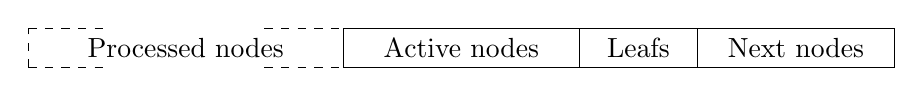
\begin{tikzpicture}[y=0.5cm, x=0.5cm]
    \draw[dashed] (0,1) -- (2,1);
    \draw[dashed] (0,0) -- (0,1);
    \draw[dashed] (0,0) -- (2,0);
    \draw (4,0.5) node {Processed nodes};
    \draw[dashed] (6,1) -- (8,1);
    \draw[dashed] (6,0) -- (8,0);
    \draw (8,1) -- (8,0);

    \draw (8,1) -- (22,1);
    \draw (8,0) -- (22,0);

    \draw (11,0.5) node {Active nodes};
    \draw (14,1) -- (14,0);

    \draw (15.5,0.5) node {Leafs};
    \draw (17,1) -- (17,0);

    \draw (19.5,0.5) node {Next nodes};
    \draw (22,1) -- (22,0);

  \end{tikzpicture}
  \caption{The structure of the kd-trees nodes in memory.}
  \label{fig:nodeStructure}
\end{figure}

% Use GPU for computations and let CPU handle minor book keeping.

As described in \refsection{sec:reduce}, our reduction algorithm
assumes that the length of the input list is a power of 2. Triangles
associated with a node are therefore split into segments with a
fixed-size that is a power of 2. Having fixed-size segments will also
make it easy to choose a kernels block size, so that each segment is
processed by one block. A segment contains information about which
triangles it contains, which node its triangles are associated with
and if there are not enough triangles to fill it, then it also stores
how many triangles it actually contains.

Performing two reductions to the triangles in the segments, once with
operator \textbf{min} and identity element $\infty$ and then with
operator \textbf{max} and identity element $-\infty$, yields the
bounding boxes of each segment. Performing a segmented reduction on
the list of segments, as describe on Algorithm 3 in \zhou, will
compute a tight bounding box for each node in activeList. This
bounding box can then be used by the spatial median splitting method
to determine where to place the splitting plane.

With the splitting plane decided for each node, the triangle/node
association can be computed by any of the methods described in
\refsection{sec:splittingSchemes}. An array of size $2 * \|triangles\|$,
$associateSide$, is used to store triangle/node
associations. Computing the prefix-sum of $associateSide$ will then
produce the addresses that each triangle should be moved to, in order
to be stored sequentially with the other triangles associated with the
same new node as it is.

\fixme{Example?}

%% Instead of reducing the sizes of child nodes, as done in \zhou{} I
%% propose a method for calculating them directly. This leads to lots
%% of uncoalesced lookups, so argue if the GPU is able to properly hide
%% these.

With the new addresses of the triangles computed, the nodes must now
be split into child nodes. For node $n$, the values in $associateAddr$
can be used to calculate the triangle index and range of the child
nodes, $left$ and $right$, as seen in \refalg{alg:childIndices}. The
idea behind \refalg{alg:childIndices} is that using the parent nodes
triangle index we are able to extract the triangle index of its left
and right child nodes. Then by adding the parents triangle amount to
its index, we can lookup the starting index of the next child nodes
triangles. Subtracting these two values yields the range of triangles
spanned by a child node.

\begin{algorithm}
  \caption{Compute child node triangle index and range}
  \label{alg:childIndices}
  \begin{algorithmic}
    \PROCEDURE{ChildTriangleInformation}
              {$parent, left, right$: Node, $associateAddr$ : List}
              {$left$ : Node, $right$ : Node}{
                \ASSIGN{$left.triangleIndex$}{$associateAddr[parent.triangleIndex]$}
                \ASSIGN{$leftEndAddr$}{$associateAddr[parent.triangleIndex + parent.triangleRange]$}
                \ASSIGN{$left.triangleIndex$}{$leftEndAddr - left.triangleIndex$}
                \ASSIGN{$right.triangleIndex$}{$associateAddr[parent.triangleIndex + \|triangles\|]$}
                \ASSIGN{$rightEndAddr$}{$associateAddr[parent.triangleIndex + parent.triangleRange]$}
                \ASSIGN{$right.triangleIndex$}{$rightEndAddr - right.triangleIndex$}
              }
  \end{algorithmic}
\end{algorithm}

Finally the triangles are moved to their new location defined by
$associateAddr$ and the algorithm has completed one iteration.





% Building the upper nodes mostly consist of moving data around, and
% not necessarily in a coalesced fashion. This makes it hard to hide
% the latency and will impact performance.

% Argue it can be done in O ( N log N )



\subsubsection{Adding empty space maximizing}\label{sec:gpuEmptySpace}

% Plugable solution, add the new nodes after the ones in nextlist.

To experiment with empty space maximization it needs to be implemented
as a plugable solution, which can be turned on and off at will. This
has been achieved with the design found in
\refalg{alg:emptySpaceMaximizing}, which injects new nodes created by
empty space maximizing into the tree. In order to perform empty space
maximizing a \textit{loose bounding box} needs to be propagated down
the tree. A loose bounding box is calculated by splitting a parents
bounding box with its splitting plane and propagated downwards to the
nodes two child nodes. Since the geometry inside a child might not
touch all sides of a parents bounding box, this propagated bounding
box provides a loose upper bound on the geometry.

\begin{algorithm}
  \caption{Calculate Empty Space Maximization}
  \label{alg:emptySpaceMaximizing}
  \begin{algorithmic}
    \PROCEDURE{CreateUpperNodes}
               {\VAR{activeNodes} : Node List}
               {\VAR{leafs,nextNodes} : Node List}{

                 \COMMENTIT{First split all triangles into segments.}
                 \STATE{...}
                 \COMMENTIT{Then compute each triangles bounding box
                   using reduction as described in
                   \refsection{sec:reduce}.}
                 \STATE{...}

                 \STATE{}
                 \COMMENTIT{Perform empty space maximization.}
                 \IF{$performEmptySpaceMaximization$}
                 \DECLARE{$emptySplitNodes, emptyAddr$}{List}
                 \DECLARE{$emptySides$}{Plane List}
                 \PARALLELFOR{$node$}{$activeList$}
                 \ASSIGN{$emptySplits[i]$}{$0$}
                   \FOREACH{$side$}{$node.boundingBox$}
                     \IF{$node$ has more than $C_e$ empty space on $side$}
                       \ASSIGN{$emptySplitNodes[i]$}{$emptySplitNodes[i] + 2$}
                       \STATE{$emptySides[node]$.Add($side$)}
                     \ENDIF
                   \ENDFOR
                 \ENDFOR
                 \ASSIGN{$emptyAddr$}{\textbf{Prefix-Sum}($emptySplitNodes$)}
                 \PARALLELFOR{$node$}{$activeList$}
                   \STATE{Cut of empty space and place new nodes
                     sequentially at addresses specified in
                     $emptyAddr$. Then rewire parent nodes to point to
                     new nodes.}
                 \ENDFOR
                 \ENDIF

                 \STATE{}
                 \COMMENTIT{Compute the addresses to move the
                   triangles to by comparing them to the splitting
                   plane.}
                 \STATE{...}
                 \COMMENTIT{Move the triangles.}
                 \STATE{...}

                 \COMMENTIT{Split nodes.}
                 \STATE{...}
  }
  \end{algorithmic}
\end{algorithm}

% Explain

The algorithm in \refalg{alg:emptySpaceMaximizing} for performing
empty space splitting is inserted right after the nodes new tight
bounding boxes have been computed and before the new child nodes are
created. If empty space maximization should be performed on one of the
nodes in activeNodes can be checked in parallel. Each side of a node
is then checked sequentially and if it is found that the amount of
empty space between the tight bounding box and the loose bounding box
on a given side is above a certain threshold, then that side is added
to the $emptySides$ list. Each empty split results in two new nodes,
one node that refers to the empty space and one node linking the
parent node with its child node. This is depicted in
\reffig{fig:emptySpaceExample}.

Once the amount of empty splits per node has been decided, where to
place those nodes is computed by calculating the prefix-sum of
$emptySplitNodes$. Empty space maximization nodes are injected into to
the list of nodes shown in \reffig{fig:nodeStructure} as describe on
\reffig{fig:emptyNodeStructure}, which again preserves the invariant
that the next batch of active nodes are located at the end of the
list.

\begin{figure}
  \centering
  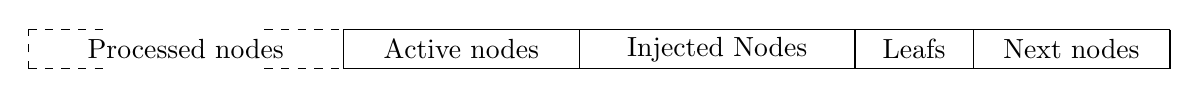
\begin{tikzpicture}[y=0.5cm, x=0.5cm]
    \draw[dashed] (0,1) -- (2,1);
    \draw[dashed] (0,0) -- (0,1);
    \draw[dashed] (0,0) -- (2,0);
    \draw (4,0.5) node {Processed nodes};
    \draw[dashed] (6,1) -- (8,1);
    \draw[dashed] (6,0) -- (8,0);
    \draw (8,1) -- (8,0);

    \draw (8,1) -- (29,1);
    \draw (8,0) -- (29,0);

    \draw (11,0.5) node {Active nodes};
    \draw (14,1) -- (14,0);

    \draw (17.5,0.5) node {Injected Nodes};
    \draw (21,1) -- (21,0);

    \draw (22.5,0.5) node {Leafs};
    \draw (24,1) -- (24,0);

    \draw (26.5,0.5) node {Next nodes};
    \draw (29,1) -- (29,0);

  \end{tikzpicture}
  \caption{The structure of the kd-trees nodes in memory with empty
    space maximization.}
  \label{fig:emptyNodeStructure}
\end{figure}


% Propagating aabb's downwards

With the addresses of the nodes produced by empty space maximization
computed, a kernel can be launched that creates the actual empty space
nodes and rewires the parent node to point to the empty space nodes
instead of its current child node. 

This construction is very flexible and all copmutations needed by
empty space maximization can be turned on and off at will, which
allows me to easily compare the quality and construction speed of
trees with and without this optimization.

\subsection{Lower Tree Creation}\label{sec:lowerNodes}

Compared with the upper tree creation phase, the lower tree creation
is quite simple and only requires a few kernels. Since there can be
thousands of nodes at the lower node phase, parallization can
effectively be done over nodes instead of primitives. 

\zhou{} proposes that the Surface Area Heuristic is used when deciding
which splitting plane to use and that the set of splitting candidates
is precomputed. Precomputing the splitting candidates instead of
clipping them after each new split can cause false primitives to
accumulate in nodes over successive splits, as described in
\refsection{sec:splittingPlane}. \zhou's reasoning is

\quotebook{While clipping is effective for large nodes by preventing
  false postives from accumulating over future splits, our experiments
  indicate that clipping rarely improves ray tracing
  performance.}{1409079}

Later in this section I will propose two simplifications to the
standard SAH approach. These simplifications may both produce
acceleration structures of lower quality than the computationally
heavy SAH, but they make up for this by being much faster.

\subsubsection{Lower Tree Splitting Planes}

% Explain the Plane struct

Before splitting any nodes however, the splitting plane structure used
in the lower node phase must be explained. To efficiently compute the
size of a nodes triangle set and sorting a nodes triangles in one
instruction, I adopt \zhou's novel approach of storing the triangle
set of a node, $n$ as an index, $i$, and a bit mask, $b$. If the
$k$'th bit in $b$ is set, this means that the $i+k$'th triangle in the
list of all triangles is associated with the node. Recall from earlier
that a node stored the reference to its associated triangles as an
index, $i$ and a range, $r$. The bit mask corrosponding to $r$ would
then simply have all it's first $r$ bits set. A more thorough example
is given in \reffig{fig:bitmap}.

\newcommand{\nodeBitmap}[5]{
  \begin{tabular}{c}
    #1 \\ 
    \begin{tikzpicture}[y=0.4cm, x=.4cm,font=\sffamily]
      \draw (0,0) -- (4,0);
      \draw (0,1) -- (4,1);
      \draw (0,0) -- (0,1);
      \draw (1,0) -- (1,1);
      \draw (2,0) -- (2,1);
      \draw (3,0) -- (3,1);
      \draw (4,0) -- (4,1);
      
      #2
      #3
      #4
      #5
    \end{tikzpicture}
  \end{tabular}
}

\begin{figure}
  \centering
  \subfloat[]{
    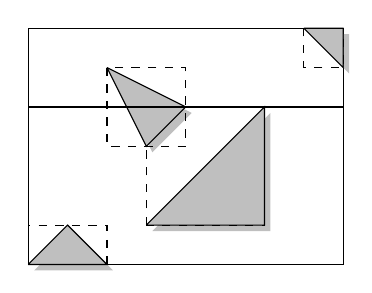
\begin{tikzpicture}[y=0.5cm, x=.5cm,font=\sffamily]
      \draw (0,0) -- (0,6) -- (8,6) -- (8,0) -- (0,0);

      \drawTri{0,0}{2,0}{1,1}
      \drawAabb{0,0}{0,1}{2,1}{2,0}
      \drawTri{3,1}{6,1}{6,4}
      \drawAabb{3,1}{3,4}{6,4}{6,1}
      \drawTri{7,6}{8,6}{8,5}
      \drawAabb{7,6}{8,6}{8,5}{7,5}
      \drawTri{2,5}{3,3}{4,4}
      \drawAabb{2,5}{2,3}{4,3}{4,5}

      \draw (0,4) -- (8,4);
    \end{tikzpicture}
  }
  \subfloat[]{
    \begin{tikzpicture}[y=0.5cm, x=.5cm,font=\sffamily,
        level/.style={sibling distance=50mm/#1}]
      \node [node] {\nodeBitmap{0}
        {\drawTri{0.2,0.3}{0.5,0.6}{0.8,0.3}}
        {\drawTri{1.2, 0.8}{1.5, 0.2}{1.8, 0.5}}
        {\drawTri{2.2,0.2}{2.8,0.2}{2.8,0.8}}
        {\drawTri{3.2, 0.8}{3.8, 0.8}{3.8, 0.2}}}
      child {node [leaf] {\nodeBitmap{1}
          {\drawTri{0.2,0.3}{0.5,0.6}{0.8,0.3}}
          {\drawTri{1.2, 0.8}{1.5, 0.2}{1.8, 0.5}}
          {\drawTri{2.2,0.2}{2.8,0.2}{2.8,0.8}}{}}}
      child {node [leaf] {\nodeBitmap{2}{}
          {\drawTri{1.2, 0.8}{1.5, 0.2}{1.8, 0.5}}{}
          {\drawTri{3.2, 0.8}{3.8, 0.8}{3.8, 0.2}}}};
    \end{tikzpicture}
  }
  \caption[A description of storing triangles as bit masks.]{A
    description of storing triangles as bit masks. The bit masks are
    represented by a grid containing triangles. If a grid cell
    contains a triangle, then that bit is set. Node 0 contains all
    triangles, as evidenced by its bit mask. Node 0 is then split
    along the splitting plane drawn in the scene, which has left
    triangle mask $[1,1,1,0]$ and right mask $[0,1,0,1]$. The result
    of splitting is leafs 1 and 2, whose triangle set is the result of
    a bitwise $and$ between Node 0's bit mask and the left and right
    bitmask respectively.}
  \label{fig:bitmap}
\end{figure}

% Example of how to store splitting planes as bitmasks

\begin{algorithm}
  \caption{Preprocess Lower Nodes.}
  \label{alg:calcSplittingPlanes}
  \begin{algorithmic}
    \PROCEDURE{PreprocessLowerNodes}
              {$upperLeafs$ : Node List}
              {$splittingPlanes$ : Plane List}{
                \PARALLELFOR{$node$}{$upperLeafs$}
                  \PARALLELFOR{$triangle$}{$node.Triangles$}
                    \ASSIGN{$aabb_p$}{GetAabb($triangle$)}
                    \COMMENTIT{Create the splitting plane sets along the x-axis.}
                    \DECLARE{$x_{low}, x_{high}$}{Plane}
                    \FOREACH{$triangle$}{$node.Triangles$}
                      \ASSIGN{$aabb_t$}{GetAabb($triangle$)}
                      \ASSIGN{$x_{low}.left[triangle]$}{$aabb_t.min.x <= aabb_p.min.x$}
                      \ASSIGN{$x_{low}.right[triangle]$}{$aabb_p.min.x < aabb_t.max.x$}
                      \ASSIGN{$x_{high}.left[triangle]$}{$aabb_t.min.x <= aabb_p.max.x$}
                      \ASSIGN{$x_{high}.right[triangle]$}{$aabb_p.max.x < aabb_t.max.x$}
                    \ENDFOR
                    \STATE{$splittingPlanes$.Add($x_{low}$)}
                    \STATE{$splittingPlanes$.Add($x_{high}$)}
                    \STATE{...}
                    \COMMENTIT{Perform similar plane constructions for the y and z axis.}
                    \STATE{...}
                  \ENDFOR
                \ENDFOR
              }
  \end{algorithmic}
\end{algorithm}

% Using shared memory


\subsubsection{SAH Tree Construction}

% Adds surface area computation to the preprocess

\begin{algorithm}
  \caption{Calculate SAH cost}
  \label{alg:calcSAHCost}
  \begin{algorithmic}
    \PROCEDURE{ComputeSAHCost}
              {$activeNodes$ : Node List}
              {$splittingPlanes$ : Plane List, $leafs$ : Boolean List}{
                \COMMENTIT{Calculate SAH for each split candidate and
                  return the split candidate with minimal SAH.}
                \PARALLELFOR{$node$}{$activeNodes$}
                  \FOREACH{split candidate $s$}{$node.splitCandidates$}
                    \ASSIGN{$bmp_L$}{$node.triangles \cap s.left$}
                    \ASSIGN{$C_L$}{$\parallel bmp_L \parallel$}
                    \ASSIGN{$A_L$}{summed surface area of $bmp_L$}
                    \ASSIGN{$bmp_R$}{$node.triangles \cap s.right$}
                    \ASSIGN{$C_R$}{$\parallel bmp_R \parallel$}
                    \ASSIGN{$A_R$}{summed surface area of $bmp_R$}
                    \ASSIGN{$weightedArea$}{$C_L * A_L + C_R * A_R$}
                  \ENDFOR
                  \ASSIGN{$splittingPlanes[node] \leftarrow p$}{Split candidate with minimal weighted area}
                  \ASSIGN{$SAH$}{$p.weightedArea / node.summedArea + C_N$}
                  \ASSIGN{$leafs[node]$}{$SAH < C_{leaf}$}
                \ENDFOR
              }
  \end{algorithmic}
\end{algorithm}

% Explain

% Run prefix sum on leafList and use the result as addresses for the
% children.

% When moving from upper nodes to lower nodes. Calculate a new tight
% bounding box inside the modified bounding box. Then approximate the
% new surface area by the reduction in BB volume.


\subsubsection{Balanced Tree Construction}

% SAH is slow, so explore alternatives.

% Testing shows that 'large' leaf node improves performance, cite Horn
% about why.

% Means that lower nodes will only be split 1-2 times and then
% intersected, ie the lower splitting planes don't need to be placed
% optimally.

% Introducing the balanced split.

\begin{algorithm}
  \caption{Calculate balanced split}
  \label{alg:calcBalancedCost}
  \begin{algorithmic}
    \PROCEDURE{ComputeBalancedSplit}
              {$activeNodes$ : Node List}
              {$splittingPlanes$ : Plane List, $leafs$ : Boolean List}{
                \COMMENTIT{Compute the relation between left and right
                  triangles for each split candidate and return the
                  candidate with best relation and presumably lowest
                  subtrees.}
                \PARALLELFOR{$node$}{$activeList$}
                  \ASSIGN{$p$}{$noSplitCandidate$}
                  \FOREACH{split candidate $s$}{$node.splitCandidates$}
                    \ASSIGN{$bmp_L$}{$node.triangles \cap s.left$}
                    \ASSIGN{$C_L$}{$\parallel bmp_L \parallel$}
                    \ASSIGN{$bmp_R$}{$node.triangles \cap s.right$}
                    \ASSIGN{$C_R$}{$\parallel bmp_R \parallel$}
                    \ASSIGN{$largestSubtree$}{\MAX{$C_L$}{$C_R$}}
                    \ASSIGN{$smallestSubtree$}{\MIN{$C_L$}{$C_R$}}
                    \IF{$largestSubtree < p.largestSubtree$ \textbf{or} \\
                      $(largestSubtree = p.largestSubtree$ \textbf{and} $smallestSubtree < p.smallestSubtree$}
                      \ASSIGN{$p$}{$s$}
                    \ENDIF
                  \ENDFOR
                  \ASSIGN{$splittingPlanes[node]$}{$p$}
                  \ASSIGN{$leafs[node]$}{$(p.largestSubtree + p.largestSubtree) / 2 + C_N < C_{leaf}$}
                \ENDFOR
              }
  \end{algorithmic}
\end{algorithm}

% Explain

\subsubsection{No Tree Construction}




% Ray tracing structures on the GPU has been mapped more or less 100%
% from CPU structures. We need to build them for the GPU instead. That
% means rethinking some of the algorithms (like add persistent
% threads.)



\chapter{Ray Tracing}\label{chp:rayTracing}

\chapterquote{Some argue that in the very long term, rendering may best be
  solved by some variant of ray tracing, in which huge numbers of rays sample
  the environment for the eye’s view of each frame. And there will also be
  colonies on Mars, underwater cities, and personal jet packs.}{Tomas Möller and
  Eric Haines}


% Motivate!

% An optimized ray tracer will be used to test whether or not more time
% spent on creating a better kD tree will pay off in final rendering
% time.

In this chapter we shall look at how to implement a ray tracer and how it can be
optimized to run efficiently on GPUs using NVIDIA's CUDA framework. The result
will be an optimized ray tracer, which will be used in \refchapter{chp:results}
to evaluate the quality of kd-trees.

A ray, $r$, is defined as a line which starts at a point called \textit{origin},
$r_{ori}$, and can be traced infinitely along a certain \textit{direction},
$r_{dir}$. Using $t$ to describe the distance traveled along the ray, $r$ can
then be described as $r(t) = t \cdot r_{dir} + r_{ori}$. Tracing a ray into the
scene to find the nearest intersecting triangle, then means finding the triangle
that the ray intersects at the lowest value of $t$. Before the actual ray
tracing can be performed, the primary rays traced from the camera and into the
scene must be computed and stored as a list of rays, $rays$. How these rays are
generated is a large topic in itself and lies outside the scope of this
thesis. Chapter 6 in \citebook{PBR:2010} provides good insight into the theory
needed for creating the primary rays.

The general structure for a ray tracer that handles reflective surfaces can be
seen in \refalg{alg:generalRayTracer}. \Refalg{alg:generalRayTracer} takes as
input a list of rays to be traced, $rays$, the scene that should be ray traced,
$scene$, and the image, $pixels$, on which the ray traced scene should be
drawn. Each ray is independent of the other rays and can therefore be traced in
parallel by the GPU. The algorithm first determines which of the triangles
intersected by the ray is closest to the ray's origin, i.e. the triangle first
\textit{seen} by the ray. It then computes the color of the triangle intersected
by the ray and blends that color with the color that has been accumulated so far
in $pixels[r]$. How the color is computed is not relevant to the kd-tree
evaluations in \refchapter{chp:results} and is therefore not discussed in this
thesis. Suffice it to say that the ray tracer produced as part of the thesis
uses the \textit{general lighting equation} described on page 83 in
\citebook{RTR2}. Finally the algorithm checks if a triangle is reflective and if
so then a reflection ray is generated and added to the $nextRays$ list. A
reflection ray's direction, $ref_{dir}$ is calculated from the triangle's
normal, $n$, and the incoming rays direction, $ray_{dir}$

\begin{displaymath}
  ref_{dir} = -2 (n \cdot ray_{dir}) n + ray_{dir}
\end{displaymath}

The new origin of the reflection ray is simply the intersection point of the
incoming ray and the triangle. As long as one or more reflection rays are
generated by the traced rays, the ray tracing process is repeated.

\begin{algorithm}
  \caption{A general ray tracer.}
  \label{alg:generalRayTracer}
  \begin{algorithmic}
    \PROCEDURE{RayTracer}
              {$rays$ : Ray List, $scene$ : Scene Description, $pixels$ : Image}
              {$pixels$ : Image}{
                \PARALLELFOR{$r$}{$rays$}
                  \COMMENTIT{The scene description can be either a list of
                    triangles in the scene, or a kd-tree created from those
                    triangles.}
                  \ASSIGN{$triangle$}{ClosestIntersectingTriangle$(r, scene)$}
                  \ASSIGN{$pixels[r]$}{ComputeColor$(pixels[r], r, triangle)$}
                  \DECLARE{$nextRays$}{Ray List}
                  \IF{IsReflective$(triangle)$}
                    \STATE{$nextRays$.Add(GenerateReflectionRay$(triangle, ray)$)}
                  \ENDIF
                \ENDFOR
                \IF{$nextRays$.NotEmpty}
                  \ASSIGN{$pixels$}{RayTracer$(nextRays, scene, pixels)$}
                \ENDIF
              }
  \end{algorithmic}
\end{algorithm}

In this chapter I will present two methods for determining which triangle in a
scene a ray intersects. In \refsection{sec:exhaustive} I present an exhaustive
ray tracer, which finds the closest intersection point by intersecting each ray
with every triangle. In \refsection{sec:hierarchicalTraversal} I then present a
hierarchical ray tracer, which will use the kd-tree to minimize the number of
triangles each ray needs to be intersected with. In the same section I will
describe three optimizations that can be applied to hierachical ray tracers
running on GPUs. The optimizations will be added incrementally to the
hierarchical ray tracer and implementation details to each specific optimization
is therefore discussed alongside the theory. The optimized ray tracer will use
the \textit{short-stack} optimization from \horn, a \textit{packet scheme}
inspired by Wald et al.\citebook{Wald:2001:IRCRT} and an optimization inspired
by Empty Space Maximization, that utilizes a leaf node's bounding box, which is
computed while creating the kd-tree.

In \refsection{sec:exhaustive} and \refsection{sec:hierarchicalTraversal} I will
merely have assumed that a method exists for determining if and where a ray and
a triangle intersects. In the final section of this chapter I will discuss two
such methods with respect to the GPU's memory hierarchy and maximizing
occupancy.

The ray tracers and their optimization will be evaluated in
\refchapter{chp:results} and hopefully show that the hierarchical ray tracer is
faster than the exhaustive ray tracer. This will be a very important result, as
the time spent rebuilding acceleration structures for dynamic scenes would
otherwise be wasted.




\section{Exhaustive Ray Tracing} \label{sec:exhaustive}

Before directing our focus on hierarchical ray tracers, we will first
take a look at an exhaustive ray tracer.

% GPU does bruteforcing well.

The reason that an exhaustive ray tracer is interesting is that the GPU comes
with high computational power, but little tolerance for branching, as was
discussed in \refsection{sec:threadHierarchy}. An exhaustive ray tracer fits
very well onto such an architecture, since intersecting each ray with every
triangle certainly requires a lot of computational power, and every ray in a
warp will loop over the same triangles and therefore not branch independently.

%, so the triangle-loop will not cause thread divergence.

% Algorithm

The ClosestIntersectingTriangle procedure used by \refalg{alg:generalRayTracer}
is implemented in \refalg{alg:exhaustive} using an exhaustive ray tracer. The
actual ray tracers implemented in this thesis also compute and return a ray's
barycentric coordinates on the triangle it intersects, which is explained in
\refsection{sec:intersection}. The barycentric coordinates are used to perform
lighting calculations, but in order to keep the algorithms simple and
instructive, this has been omitted and is assumed to be performed by the
ComputeColor method invoked in \refalg{alg:generalRayTracer}.


\begin{algorithm}
  \caption{An exhaustive implementation of ClosestIntersectingTriangle}
  \label{alg:exhaustive}
  \begin{algorithmic}
    \PROCEDURE{ClosestIntersectingTriangle}
              {$R$ : Ray, $Ts$, Triangle List}
              {$t_{near}$ : Triangle}{
                \ASSIGN{$t_{near}$}{$NULL$}
                \FOREACH{$t$}{$Ts$}
                  \ASSIGN{$t_{near}$}{ClosestHit$(t, t_{near})$}
                \ENDFOR
              }
  \end{algorithmic}
\end{algorithm}

The downside to the exhaustive approach is that intersecting a ray with $m$
triangles, yields a time complexity of $O(m)$.

\section{Hierarchical Ray Tracing}\label{sec:hierarchicalTraversal}

% Time complexity of O(n log m)

Hierarchical ray tracers provide a better upper bound than exhaustive ray
tracers. Given a hierachical data structure over $m$ geometric primitives in a
scene, the leaf node that a ray should traverse next can be found in $O(\log m)$
time. This is significantly better than the exhaustive ray tracer from
\refsection{sec:exhaustive}.

% Describe how the tree is traversed

When ray tracing a scene using a kd-tree as acceleration structure, each ray
traverses the tree in search of the leaf node closest to the rays origin, while
still being in front of the ray. The leaf nodes is hereafter refered to as the
\textit{nearest leaf}. At each interior node, the ray needs to determine which
of the child nodes it should traverse next. This process is continued until a
leaf node is reached. The ray then needs to intersect each triangle in the leaf
and determine which intersected triangle is nearest, if any. If the ray
intersects a triangle, then it reports this intersection, otherwise it needs to
continue traversing the tree. How this is done is the topic of
\refsection{sec:kdRestart} and \refsection{sec:shortStack}. The general
algorithm for ray tracing a kd-tree can be seen in \refalg{alg:generalTracing}.

\begin{algorithm}
  \caption{A general kd-tree traversal algorithm for ray tracing}
  \label{alg:generalTracing}
  \begin{algorithmic}
    \PROCEDURE{ClostestIntersectingTriangle}
              {$ray$ : Ray, $tree$ : kd-tree}
              {$t_{near}$ : Triangle}{
                \ASSIGN{$t_{near}$}{$NULL$}
                \WHILE{ray inside scene}
                  \COMMENTIT{Traverse the tree until the leaf node nearest the
                    ray origin is found and store the distance to the nearest
                    splitting plane the ray intersects in $d_{split}$.}
                  \ASSIGN{$(leaf, d_{split})$}{TraverseTree($ray, tree$)}
                  \COMMENTIT{Intersect triangles in leaf and return the nearest
                    intersected triangle, if any.}
                  \ASSIGN{$t_{near}$}{Intersect($ray, leaf.triangles$)}
                  \COMMENTIT{Break if a closest intersection
                    is found and return it.}
                  \IF{$t_{near} \neq NULL$}
                    \STATE{\textbf{break}}
                  \ELSE
                    \ASSIGN{$ray.origin$}{$ray.origin + d_{split} * ray.direction$}
                  \ENDIF
                \ENDWHILE
              }
  \end{algorithmic}
\end{algorithm}

% Traversal method

The method used to determine which of an interior node's children to visit next
can be seen in \refalg{alg:generalTraversal}. For each interior node the ray
first needs to determine which of the two children are placed \textit{nearest}
and \textit{farthest} along the rays direction. It then computes the signed
distance from the ray to the nodes splitting plane. If this distance is below 0
then the plane is located behind the ray and the farthest child must be
visited. If the distance is above 0 then the nearest node needs to be visited
next. In addition the distance, $d_{split}$, to the nearest splitting plane in
front of the ray needs to be updated. $d_{split}$ is used to advance the ray
beyond a visited leaf node if it did not intersect any geometry.

\begin{algorithm}
  \caption{A basic kd-tree traversal algorithm}
  \label{alg:generalTraversal}
  \begin{algorithmic}
    \PROCEDURE{TraverseTree}
              {$ray$ : Ray, $tree$ : kd-tree}
              {$leaf$ : Node, $d_{split}$ : Number}{
                \ASSIGN{$d_{split}$}{$\infty$}
                \ASSIGN{$node$}{$tree.root$}
                \WHILE{$node \neq LEAF$}
                  \COMMENTIT{The signed distance to the nodes splitting plane.}
                  \ASSIGN{$node_{near}$}{$ray.direction[node.axis] > 0$ ? $node.left$ : $node.right$}
                  \ASSIGN{$node_{far}$}{$ray.direction[node.axis] > 0$ ? $node.right$ : $node.left$}
                  \ASSIGN{$d_{node}$}{($node.splitValue - ray.origin[node.axis]) / ray.direction[node.axis]$}
                  \IF{$0 < d_{split}$}
                    \ASSIGN{$node$}{$node_{near}$}
                    \ASSIGN{$d_{split}$}{min$(d_{split}, d_{node})$}
                  \ELSE
                    \ASSIGN{$node$}{$node_{far}$}
                  \ENDIF
                \ENDWHILE
              }
  \end{algorithmic}
\end{algorithm}

In \reffig{fig:simpleScene} a simple scene consisting of four triangles is
shown. The corrosponding kd-tree matching the axis aligned splitting planes is
shown in \reffig{fig:simpleTree}. A tree traversal of the ray, $r(t) = t
\vectwoT{2}{1} + \vectwoT{0}{1}$, entering the scene in the lower left would
look like this: Upon entering the scene the ray first visits the root node,
0. Node 0 splits the scene along the x-axis at $x=4$ and the rays distance to
that plane is then $d_{split} = (4 - 0) / 2 = 2$. The ray therefore proceeds to
the childnode $2 > 0$ ? $1$ : $2 = 1$. The signed distance to node 1's splitting
plane is $d_{node} = (4 - 1) / 1 = 3$ and the ray proceeds to node $1 > 0$ ?
$3$ : $2 = 3$, where it finds no primitives to intersect. The ray is then
advanced beyond the nearest splitting plane by advancing it $d_{split}$ along
its direction. The new ray becomes $r'(t) = r(t) + d_{split} \cdot r_{dir} =
r(t) + 2 \vectwoT{2}{1} = t \vectwoT{2}{1} + \vectwoT{4}{3}$. Since the ray did
not intersect any geometry and has not advanced beyond the scene, the traversal
process is restarted for $r'(t)$.


\begin{figure}
  \centering
  \subfloat[A simple scene subdivided by a kd-tree.]{
    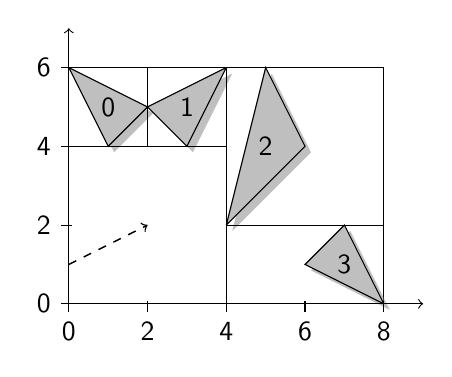
\begin{tikzpicture}[y=0.5cm, x=0.5cm,font=\sffamily]
      \drawNode{0,0}{8,0}{8,6}{0,6}

      % Tris
      \drawTri{0,6}{1,4}{2,5}
      \draw (1,5) node{0};
      \drawTri{4,6}{3,4}{2,5}
      \draw (3,5) node{1};
      \drawTri{4,2}{5,6}{6,4}
      \draw (5,4) node{2};
      \drawTri{8,0}{7,2}{6,1}
      \draw (7,1) node{3};

      % Splits
      \draw (4,0) -- (4,6);
      \draw (0,4) -- (4,4);
      \draw (2,4) -- (2,6);
      \draw (4,2) -- (8,2);

      % Ray
      \drawRay{0,1}{2,2}

      %axes
      \draw[->] (0,0) -- coordinate (x axis mid) (9,0);
      \draw[->] (0,0) -- coordinate (y axis mid) (0,7);
      %ticks
      \foreach \x in {0,2,...,9}
     		\draw (\x,1pt) -- (\x,-3pt)
			node[anchor=north] {\x};
    	\foreach \y in {0,2,...,7}
     		\draw (1pt,\y) -- (-3pt,\y) 
     			node[anchor=east] {\y}; 
    \end{tikzpicture}
    \label{fig:simpleScene}
  }
  \hspace{20pt}
  \subfloat[The kd-tree matching the scene. The gray shaded nodes represent the
    ray's traversal of the kd-tree.]{
    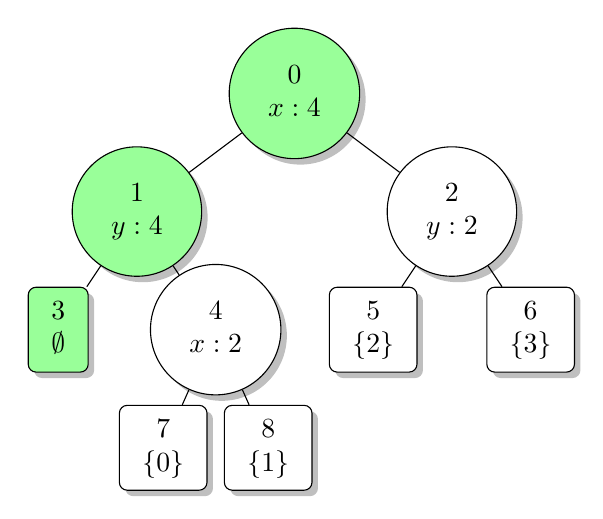
\begin{tikzpicture}[y=0.5cm, x=.5cm,font=\sffamily,
        level/.style={sibling distance=40mm/#1}]
      \node [visitedNode] (0){$\begin{array}{c}0\\x:4\end{array}$}
        child {node [visitedNode] (1) {$\begin{array}{c}1\\y:4\end{array}$}
          child {node [visitedLeaf] (e) {$\begin{array}{c}3\\\emptyset\end{array}$}}
          child {node [node] (3) {$\begin{array}{c}4\\x:2\end{array}$}            
            child {node [leaf] (e) {$\begin{array}{c}7\\\{0\}\end{array}$}}
            child {node [leaf] (e) {$\begin{array}{c}8\\\{1\}\end{array}$}}
          }
        }
        child {node [node] (2) {$\begin{array}{c}2\\y:2\end{array}$}
            child {node [leaf] (e) {$\begin{array}{c}5\\\{2\}\end{array}$}}
            child {node [leaf] (e) {$\begin{array}{c}6\\\{3\}\end{array}$}}
        };
    \end{tikzpicture}
    \label{fig:simpleTree}
  }
  \caption[A simple scene and its kd-tree.]{}
  \label{fig:simpleSceneTree}
\end{figure}


\subsection{KD-restart}\label{sec:kdRestart}

% KD restart is the simplest and fastest.

The approach presented above, where kd-tree traversal is restarted at the root
node, is known as \textit{kd-restart} and is one of the simplest algorithms for
ray tracing kd-trees. The reason for the name is that if a ray does not
intersect any triangles in the nearest leaf node, then it advances past that
leaf node using $d_{split}$ and restarts traversal from the root of the tree.

% Instead of advancing the ray simply update tMin

The algorithm in its entirety is presented in \refalg{alg:KDRestart}. Instead of
advancing the ray by updating its origin, a signed distance, $d_{min}$, is used
to determine how far a ray has traveled.

\begin{algorithm}
  \caption{A kd-restart implementation of ClosestIntersectingTriangle}
  \label{alg:KDRestart}
  \begin{algorithmic}
    \PROCEDURE{ClosestIntersectingriangle}
              {$ray$ : Ray, $tree$ : kd-tree}
              {$t_{near}$ : Triangle}{
                \ASSIGN{$t_{near}$}{$NULL$}
                \ASSIGN{$d_{min}$}{$0$}
                \WHILE{$d_{min} < \infty$}
                  \ASSIGN{$d_{split}$}{$\infty$}
                  \ASSIGN{$node$}{$tree.root$}
                  \COMMENTIT{Traverse the tree until a leaf node is reached}
                  \WHILE{$node \neq LEAF$}
                    \ASSIGN{$d_{node}$}{($node.splitPosition - ray.origin[node.axis]) / ray.direction[node.axis]$}
                    \IF{$d_{min} < d_{node}$}
                      \ASSIGN{$node$}{$ray.direction[node.axis] > 0$ ? $node.left$ : $node.right$}
                      \ASSIGN{$d_{split}$}{min$(d_{split}, d_{node})$}
                    \ELSE
                      \ASSIGN{$node$}{$ray.direction[node.axis] > 0$ ? $node.right$ : $node.left$}
                    \ENDIF
                  \ENDWHILE
                  \COMMENTIT{Test intersection with the leafs primitives}
                  \ASSIGN{$t_{near}$}{Intersect($ray, leaf.triangles$)}
                  \IF{$t_{near} \neq NULL$}
                    \STATE{\textbf{break}}
                  \ELSE
                    \COMMENTIT{Advance the ray beyond the next splitting plane.}
                    \ASSIGN{$d_{min}$}{$d_{split}$}
                  \ENDIF
                \ENDWHILE
              }
  \end{algorithmic}
\end{algorithm}

\subsection{Short-stack}\label{sec:shortStack}

% Kd-Restart traverses many of the same nodes, because 

When a ray triggers a restart in kd-restart, it will almost always traverse many
of the same interior nodes as it did in its previous traversel. The reason for
this is that kd-trees will often store spatially local nodes as local nodes in
the tree. CPU ray tracers utilize this property by pushing the not-visited child
of an interior node onto a stack and then resuming from the first node on that
stack instead of restarting. This can save a lot of resources otherwise spent on
traversing the tree, since the ray will now skip interior nodes already visited
and resume closer to the next leaf node.

CUDA's memory model, however, is not flexible enough for this approach, which
requires either dynamically allocating more memory if the stack is filled or
pre-allocating a \textit{large enough} stack in local memory to handle any given
kd-tree. This would require quite large amounts of memory for huge scenes and
might even require too much memory for practical use on today's graphics
cards. The solution proposed by \horn{} was to use a \textit{short-stack}, a
fixed-size, circular stack of $N$ elements, and then revert to using kd-restart
if the stack underflows. The circular nature of the short-stack means that the
stack will favor nodes near the leafs and overwrite nodes traversed at the top
of the kd-tree. Since the nodes near the leafs are the ones with the highest
associated traversal cost, these are exactly the ones we would like to be able
to resume from in future traversals. In their research \horn{} found that a
short-stack approach only visited 3\% more nodes compared to the unlimited stack
in CPU approaches.

% Only push usefull 'forward' nodes to the stack.

Obviously all child nodes can not be pushed onto the short-stack, as that would
force the rays to visit the entire kd-tree. Therefore restrictions need to be
formulated as to which nodes should be pushed onto the short-stack. The first
restriction is not to push nodes located behind the ray, since the ray can never
intersect these. The second restriction is not to push nodes where the distance
to the splitting plane is greater than $d_{split}$, as these would never be
visited in a kd-restart traversal. The reasoning for this is that if a ray
advances beyond the splitting plane of one of its parent nodes, it effectively
means the ray should never visit that nodes nearest subtree again and therefore
no nodes from that subtree should be stored in the short-stack. An
implementation of kd-restart with the short-stack optimization is shown in
\refalg{alg:ShortStack}.

\begin{algorithm}
  \caption{A short-stack implementation of ClosestIntersectingTriangle}
  \label{alg:ShortStack}
  \begin{algorithmic}
    \PROCEDURE{ClosestIntersectingTriangle}
              {$ray$ : Ray, $tree$ : kd-tree}
              {$t_{near}$ : Triangle}{
    \ASSIGN{$t_{near}$}{$NULL$}
    \ASSIGN{$d_{min}$}{$0$}
    \WHILE{$d_{min} < \infty$}
      \IF{$stack$.IsEmpty}
        \ASSIGN{$node$}{$tree.root$}
        \ASSIGN{$d_{split}$}{$\infty$}
      \ELSE
        \ASSIGN{$(node, d_{split})$}{$stack$.Pop}
      \ENDIF
      \COMMENTIT{Traverse the tree until a leaf node is reached}
      \WHILE{$node \neq LEAF$}
        \ASSIGN{$d_{node}$}{($node.splitPosition - ray.origin[node.axis]) / ray.direction[node.axis]$}
        \IF{$d_{min} < d_{node}$}
          \ASSIGN{$node$}{$ray.direction[node.axis] > 0$ ? $node.left$ : $node.right$}
          \IF{$d_{node} < d_{split}$}
            \STATE{stack.push($upperChild, d_{split}$)}
          \ENDIF
          \ASSIGN{$d_{split}$}{min$(d_{split}, d_{node})$}
        \ELSE
          \ASSIGN{$node$}{$ray.direction[node.axis] > 0$ ? $node.right$ : $node.left$}
        \ENDIF
      \ENDWHILE
      \COMMENTIT{Test intersection with the leafs primitives}
      \ASSIGN{$t_{near}$}{Intersect($ray, leaf.triangles$)}
      \IF{$d_{min} < t_{split}$}
        \STATE{\textbf{break}}
      \ELSE
        \COMMENTIT{Advance the ray beyond the next splitting plane.}
        \ASSIGN{$d_{min}$}{$d_{next}$}
      \ENDIF
    \ENDWHILE
              }
  \end{algorithmic}
\end{algorithm}

% Example

Let us look at a simple example of how the short-stack will speedup
traversal. Using the scene in \reffig{fig:simpleSceneTree} again, we saw
previously that the ray, $R(t) = t \vectwoT{2}{1} + \vectwoT{0}{1}$, will
traverse nodes 0, 1, and 3. At node 0 the distance to the splitting plane was 2,
meaning the splitting plane is in front and the child not traversed should be
pushed to the short-stack. At node 1 the distance was 3, so the ray intersects
node 1's splitting plane after node 0's. Node 1's other child therefore does not
need to be pushed to the stack. The result of the first traversal can be seen on
\reffig{fig:shortStack1}.

So far the short-stack traversal and kd-restart traversal have both chosen the
exact same path through the tree. But where kd-restart would have had to restart
its traversal from the root node, the short-stack allows the ray to start the
second traversal from node 2 and proceed to leaf 5, where the ray intersects
triangle 2.

In this simple example having a short-stack only allows the ray to skip one node
at the cost of maintaining and using a short-stack, which will cause a
significant overhead. Consequently having a short-stack will probably not
provide any speedup in this small example. But imagine this simple tree as a
subtree in a much larger scene, with perhaps ten levels of nodes above it. Then
a short-stack implementation allows the ray to skip those first eleven nodes,
which can yield quite a performance improvement.

\begin{figure}
  \centering

  \subfloat[The short-stack algorithm's first traversal of the scene
    from \reffig{fig:simpleSceneTree}. When the ray traversed node 0
    it pushed node 2 onto the short-stack.]{
    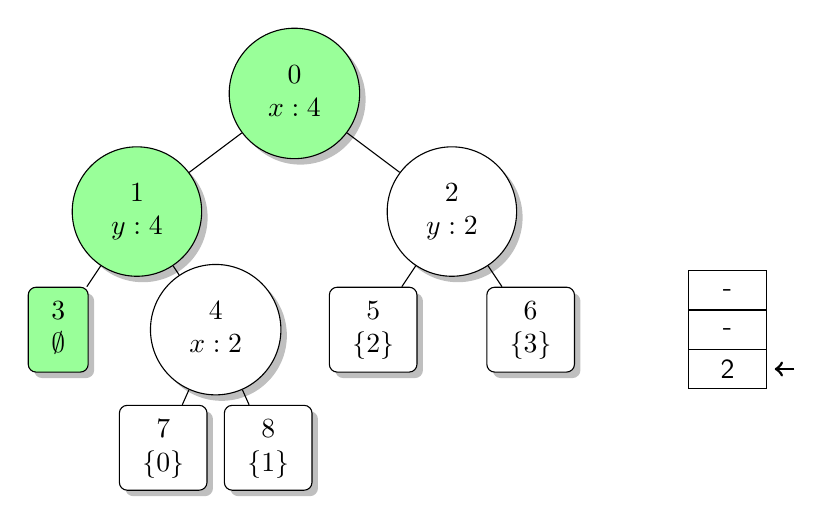
\begin{tikzpicture}[y=0.5cm, x=.5cm,font=\sffamily,
        level/.style={sibling distance=40mm/#1}]
      \node [visitedNode] (0){$\begin{array}{c}0\\x:4\end{array}$}
        child {node [visitedNode] (1) {$\begin{array}{c}1\\y:4\end{array}$}
          child {node [visitedLeaf] (e) {$\begin{array}{c}3\\\emptyset\end{array}$}}
          child {node [node] (3) {$\begin{array}{c}4\\x:2\end{array}$}            
            child {node [leaf] (e) {$\begin{array}{c}7\\\{0\}\end{array}$}}
            child {node [leaf] (e) {$\begin{array}{c}8\\\{1\}\end{array}$}}
          }
        }
        child {node [node] (2) {$\begin{array}{c}2\\y:2\end{array}$}
            child {node [leaf] (e) {$\begin{array}{c}5\\\{2\}\end{array}$}}
            child {node [leaf] (e) {$\begin{array}{c}6\\\{3\}\end{array}$}}
        };
                        
      % Short-stack
      \draw (10,-4.5) -- (10,-7.5) -- (12,-7.5) -- (12,-4.5) -- (10,-4.5);
      \draw (10, -6.5) -- (12, -6.5);
      \draw (10, -5.5) -- (12, -5.5);
      \draw (11, -7) node{2};
      \draw (11, -6) node{-};
      \draw (11, -5) node{-};
      \draw[->,line width=1pt] (12.7,-7) -- (12.2,-7);
    \end{tikzpicture}
    \label{fig:shortStack1}
  }
  \\
  \subfloat[The short-stack algorithm's second traversal of the scene
    from \reffig{fig:simpleSceneTree}. Traversal is resumed from the first
    node on the stack, which is 2.]{
    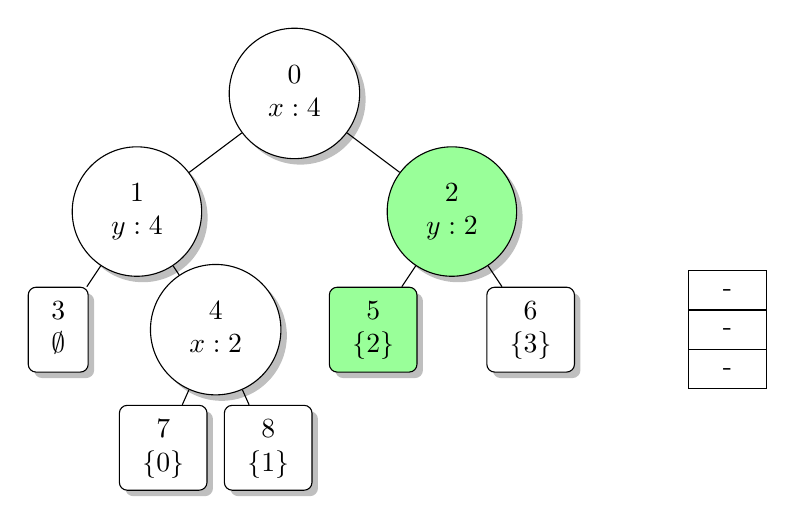
\begin{tikzpicture}[y=0.5cm, x=.5cm,font=\sffamily,
        level/.style={sibling distance=40mm/#1}]
      \node [node] (0){$\begin{array}{c}0\\x:4\end{array}$}
        child {node [node] (1) {$\begin{array}{c}1\\y:4\end{array}$}
          child {node [leaf] (e) {$\begin{array}{c}3\\\emptyset\end{array}$}}
          child {node [node] (3) {$\begin{array}{c}4\\x:2\end{array}$}            
            child {node [leaf] (e) {$\begin{array}{c}7\\\{0\}\end{array}$}}
            child {node [leaf] (e) {$\begin{array}{c}8\\\{1\}\end{array}$}}
          }
        }
        child {node [visitedNode] (2) {$\begin{array}{c}2\\y:2\end{array}$}
            child {node [visitedLeaf] (e) {$\begin{array}{c}5\\\{2\}\end{array}$}}
            child {node [leaf] (e) {$\begin{array}{c}6\\\{3\}\end{array}$}}
        };
                        
      % Short-stack
      \draw (10,-4.5) -- (10,-7.5) -- (12,-7.5) -- (12,-4.5) -- (10,-4.5);
      \draw (10, -6.5) -- (12, -6.5);
      \draw (10, -5.5) -- (12, -5.5);
      \draw (11, -7) node{-};
      \draw (11, -6) node{-};
      \draw (11, -5) node{-};
    \end{tikzpicture}
    \label{fig:shortStack2}
  }
  \caption[Short-stack kd-tree traversal.]{}
\end{figure}


\subsection{Packets}

% Packets: 2x2 packets on the CPU for to take advantage of SIMD
% instructions (Wald), warp size packets on the GPU. While
% \citebook{1230129} implemented packets, they merely assumed it would
% yield a speedup and did not provide any results. Aila2009 is against
% packets as they in practice seem to make it slower.

Using some form of \textit{packets} to accelerate ray tracing is quite a
standard technique. Packets were introduced to CPU ray tracers by Wald et
al.\citebook{Wald:2001:IRCRT}, who utilized \textit{SIMD}\footnote{Single
  instruction, multiple data.} instructions to trace rays in packets of four
rays at a time. \horn{} extended their short-stack implementation with another
form of packet tracing, where individual threads would trace multiple rays to
amortize the cost of traversing the tree. Unfortunately tracing several rays in
one thread increases thread incoherence across threads in a warp and \aila{}
concludes that

\quotebook{It is worth noticing that [kd-restart] is faster than
  packet traversal in all cases, and with diffuse rays the difference
  is approximately 2X.}{Aila2009}

% As ray tracing becomes more complex packets also become less
% effective, as rays will become more chaotic in nature and less
% likely to fit into packets.

% I will adobt a pretty cheap packet strategy: I will trace my rays in
% 4x8 packets to increase (spatial) ray coherence across warps.

While \horn's approach to packet tracing might not have yielded the intended
increase in performance, the GPU is still tracing rays in warp-sized packets and
an effective ray tracer needs to address this.

On the GPU the rays are stored in rows from left to right in a linear list. For
an image with a resolution of 64x48, processing the $n$'th ray with the $n$'th
tread results in the ray/warp classification seen in
\reffig{fig:sequentialRayWarp}, which I will call \textit{sequantial ray
  tracing}. As seen on the figure, a large number of warps are intersecting the
detailed dragon geometry. The threads in those warps who quickly intersect their
rays with the simple background will then have to idle, while waiting for the
rays intersecting the detailed dragon to finish.

Instead I propose to take advantage of the spatial coherence between
neighbouring rays and organize spatially coherent rays into warpsized packets as
done in \reffig{fig:coherentRayWarp}, where the rays are organized into packets
with a width, $p_{width}$, of 4 and a height, $p_{height}$, of 8. As the figure
demonstrates, not only does fewer warps ray trace the detailed dragon, but the
spatial coherence between the rays in a warp causes more warps to ray trace the
same spatially local geometry, which results in fewer global memory transactions
per warp.

\begin{figure}
  \subfloat[Sequential ray tracing. Notice how almost all of the
    warps overlap both the dragon and box.]{
    \begin{tikzpicture}[y=0.45cm, x=.45cm,font=\sffamily]
      \node {\includegraphics[width=7.2cm, height=5.4cm]{RefractionDragon}};
      \foreach \x in {-8,0,...,8} \draw[color=black] (\x,-6) -- (\x, 6);
      \foreach \y in {-6,-5.75,...,6} \draw[color=black] (-8,\y) -- (8, \y);
    \end{tikzpicture}
    \label{fig:sequentialRayWarp}
  }
  \hspace{20pt}
  \subfloat[Spatially coherent ray tracing. Fewer warps will now
    ray trace the dragon and the spatial coherence between rays
    results in entire warps raytracing the same side of the box.]{
    \begin{tikzpicture}[y=0.45cm, x=.45cm,font=\sffamily]
      \node {\includegraphics[width=7.2cm, height=5.4cm]{RefractionDragon}};
      \foreach \x in {-8,-7,...,8} \draw (\x,-6) -- (\x, 6);
      \foreach \y in {-6,-4,...,6} \draw (-8,\y) -- (8, \y);
    \end{tikzpicture}
    \label{fig:coherentRayWarp}
  }
  \caption[Sequantial and spatially coherent rays per warp.]{}
\end{figure}

The calculations needed to transform sequentially ordered ray ids into spatially
local ray ids are quite simple and can be seen in \refalg{alg:packet}. The
performance benefits gained by tracing spatially coherent rays and fewer global
memory transactions are enormous though, as seen in
\vreffig{fig:rayTracerEvaluation}.

It should be noted that a possibility exists that rays reflected multiple times
may eventually diverge completely and no longer be spatially coherent, but this
is no more of a problem for spatially local ray packets, than it is with the
sequential ray tracing approach and the spatially local ray packets will still
speed up primary rays.

\begin{algorithm}
  \caption{Converting a thread id to a ray id.}
  \label{alg:packet}
  \begin{algorithmic}
    \PROCEDURE{PacketID}
              {$thread$ : id}
              {$ray$ : id}
              {\COMMENTIT{Calculate the index of the packet cell.}
                \ASSIGN{$p_{id}$}{$thread / (p_{width} * p_{height})$}
                \COMMENTIT{Then compute the location of that cell in the grid of packets.}
                \ASSIGN{$grid_x$}{$p_{id} \mod  (image_{width} / p_{width})$}
                \ASSIGN{$grid_y$}{$p_{id} / (image_{width} / p_{width})$}
                \COMMENTIT{Compute the location of the ray inside that packet cell.}
                \ASSIGN{$p_x$}{$threads \mod  p_{width}$}
                \ASSIGN{$p_y$}{$(threads \mod (p_{width} * p_{height})) / p_{width}$}
                \COMMENTIT{Finally compute the location of the ray inside the grid and return the ray id.}
                \ASSIGN{$ray_x$}{$grid_x * p_{width} + p_x$}
                \ASSIGN{$ray_y$}{$grid_y * p_{height} + p_y$}
                \ASSIGN{$ray$}{$ray_x + ray_y * screen_{width}$}
              }
  \end{algorithmic}
\end{algorithm}


\subsection{Skipping Leaf Nodes}

% Inspired by Empty Space Maximization

The final ray tracer optimization presented in this thesis is inspired by the
early out option provided by Empty Space Maximization.

%% and combines the simple traversal of kd-trees with the bvh-tree's rigorous
%% intersection checks.

Since the only information available to rays traversing a kd-tree is the
position of the splitting plane and not the bounding volume of the node, the ray
can easily get sidetracked and end up in leaf nodes, whose bounding box it does
not even intersect. \Reffig{fig:waywardRay} is a simple example of
this. Extending the ray, $R(t) = t \vectwoT{1}{1} + \vectwoT{-4}{0}$, we can
clearly see that it will intersect leaf node 2. Unfortunately, when using
kd-trees, the only information available to the ray is that the node is split
along the y-axis at position 3, which in the above example causes the ray to get
sidetracked into leaf 1. This is a problem in scenes with large empty areas that
a ray has to traverse. Each time the ray intersects a splitting plane in those
empty areas, it can get sidetracked and traverse subtrees, whose associated
geometry the ray does not intersect.

%% An example of this is the great hall in the Sponza scene, where applying this
%% optimization will yield quite a performance increase, as can be seen in
%% \reffig{fig:rayTracerEvaluation}.

Empty Space Maximization has shown us that providing an early out option for
rays that would otherwise get sidetracked can increase performance
substantially. 
%and that also applies to this case. 
Since the leaf's bounding boxes are known from the tree creation phase, they can
be used to provide such an early out option and quickly skip leaf nodes that the
ray does not intersect. This saves a ray a lot of triangle intersection tests.

This optimization is only possible because I've stored the leafs bounding box
and will not be applicable in scenes where only a kd-tree is available. 

%% It does however show a major flaw in the kd-tree acceleration structure and a
%% more general solution to diverging rays will be presented under Future Work
%% in \refchapter{chp:future}.

\begin{figure}
  \centering
  \subfloat{
    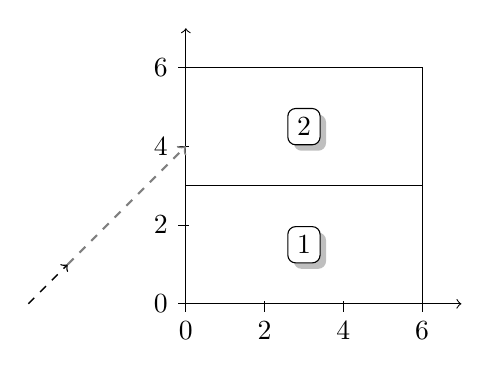
\begin{tikzpicture}[y=0.5cm, x=.5cm]
      \drawNode{0,0}{6,0}{6,6}{0,6}      

      %Splits
      \draw (0,3) -- (6,3);
      
      % Leaf names
      \draw (3,1.5) node[leaf]{1};
      \draw (3,4.5) node[leaf]{2};

      \axes{7}{7}

      \drawRay{-4,0}{-3,1}
      \draw[line width=0.75pt, dashed, ->, color=gray] (-3,1) -- (0,4);
    \end{tikzpicture}
    \label{fig:waywardScene}
  }
  \subfloat{
    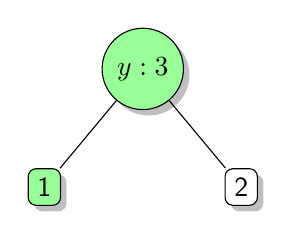
\begin{tikzpicture}[y=0.5cm, x=.5cm,font=\sffamily,
        level/.style={sibling distance=25mm/#1}]
      \node [visitedNode] (0){$y:3$}
        child {node [visitedLeaf] (1) {1}}
        child {node [leaf] (2) {2}}
        ;
    \end{tikzpicture}
    \label{fig:waywardTree}
  }
  \caption{A ray straying into a tree node, whose bounding box it does
    not intersect.}
  \label{fig:waywardRay}
\end{figure}

% Is not a general kd-tree optimization. Only works because we already
% have the bounding boxes from the tree creation phase and won't
% deallocate the space.




\section{Ray/Triangle Intersection}\label{sec:intersection}

The inherent diverging behaviour of rays traversing the kd-tree makes them hard
to parallize efficiently on the graphics card, since data access will be nearly
impossible to coalesce. The solution is to have enough active warps to
effectively hide the latency from global data fetching. This means that each
rays register usage must be kept to a minimum, in order to have enough memory
for as many active warps as possible.

Deciding which ray/triangle intersection method to use when ray tracing can
lower register usage and thus yield a significant performance boost.

% Consists of 2 parts. Ray/plane intersection which tells us the
% distance the ray will travel, and ray/triangle tests which tells us
% if the ray intersected the triangle.

Ray/triangle intersection can be broken down into two parts: A \textit{ray/plane
  intersection} test, which computes the signed distance, $t$, a ray must travel
to intersect the plane spanned by a triangle, and a \textit{triangle inclusion}
test, which checks if the intersection point is located inside the triangle. The
inclussion test is usually performed by calculating the intersection point's
\textit{barycentric coordinates} within the triangle.

Every point on a triangle, $T$, with vertices $T_a$, $T_b$ and $T_c$, can be described
as

\begin{displaymath}
  T(u,v) = (1-u-v)T_a + uT_b + vT_c, 0 \le u, 0 \le v, u+v \le 1
\end{displaymath}
 
where $(u, v)$ are the aforementioned barycentric coordinates. For a barycentric
coordinate to be inside $T$ it must therefore fulfill the requirements $0 \le
u$, $0 \le v$ and $u+v \le 1$.

Just as barycentric coordinates are used to linearly interpolate the vertex
positions across the triangle, they are also important for interpolating other
vertex attributes, such as normals or colors.

The following two ray/triangle intersection methods both compute the signed
distance and barycentric coordinates.

\subsection{Möller-Trumbore}

% One of the most popular intersection algorithms and featured in
% Real-Time Rendering.

The algorithm presented in Möller-Trumbore\citebook{MollerTrumbore97} is one of
the most popular algorithms for ray/triangle intersection, probably in no small
part due to its appearence in chapter 16.8 of Real-Time
Rendering\citebook{RTR3}, but also because it is one of the fastest ray/triangle
intersection algorithms that do not rely on extra memory or preprocessing of the
triangle before ray tracing.

% Calculates the transformation that transform the triangle into the
% unit triangle and applies this transformation to the ray.

Möller-Trumbore\citebook{MollerTrumbore97} exploits the fact that computing the
intersection between a triangle, $T(u, v)$ and ray, $R(t) = tR_{dir} + R_{ori}$ is
equivalent to solving the linear system of equations, the \textit{ray/triangle
  intersection equation}

%% The basic idea of the algorithm is to find the affine transformation
%% that, when applied to the triangle $T(u,v)$, transforms it into the unit
%% triangle, $U$, which has vertices $\vecthreeT{0}{0}{0}$,
%% $\vecthreeT{1}{0}{0}$ and $\vecthreeT{0}{1}{0}$. That affine
%% transformation is then applied to the ray, $R(t) = O + tD$, which
%% yields the vector $\vecthreeT{t}{u}{v}$, where $t$ is the distance to
%% the plane spanned by $T(u,v)$ and $u$ and $v$ are the barycentric
%% coordinates of the intersection point.

%% In short this boils down to solving the linear system of equations,
%% the \textit{ray/triangle intersection equation}

\begin{displaymath}
  \begin{array}{rl}
    & R(t) = T(u,v) \\
    \Updownarrow \\
    & tR_{dir} + R_{ori} = (1-u-v)T_a + uT_b + vT_c \\
  \end{array}
\end{displaymath}


Solving the ray/triangle intersection equation amounts to determining the signed
distance from the ray to the triangle, $t$, and the barycentric coordinates,
$(u, v)$. In \citebook{MollerTrumbore97} this is done by rearranging the terms
and applying Cramer's Rule, and the solution then becomes

\begin{displaymath}
  \vecthree{t}{u}{v} = \frac{1}{p \cdot e_1} 
  \vecthree{q \cdot e_2}{p \cdot r}{q \cdot R_{dir}}
\end{displaymath}

where $e_1 = T_b - T_a$, $e_2 = T_c - T_a$, $r = R_{ori} - T_a$, $p = R_{dir} \times  e_2$
and $q = r \times  e_1$.

\subsubsection{Implementation}

The implementation of this method is pretty straightforward using CUDA's vector
primitives and can be seen in \refalg{alg:moellerTrumbore}. The implementation
provided in \citebook{MollerTrumbore97} was optimized for the CPU and therefore
provided a lot of early out options as soon as the algorithm detected that a ray
had missed the triangle. Due to the synchonized behaviour of threads in the same
warp, providing as many early out possibilities as \citebook{MollerTrumbore97}
causes a branching overhead and results in reduced performance. This is
understandable since only one ray needs to intersect its triangle in order for
every thread in the warp to have to wait for it to finish. For the ray tracers
implemented as part of this thesis the optimal compromise was found to be only
providing one early exit after the ray/plane intersection and before computing
the barycentric coordinates.

\begin{algorithm}
  \caption{Möller-Trumbore ray/triangle intersection test}
  \label{alg:moellerTrumbore}
  \begin{algorithmic}
    \PROCEDURE{Möller-Trumbore}
              {$T$ : triangle, $R$ : ray}
              {$hit$ : bool, $t$ : distance, $(u,v)$ : barycentric coordinates}
              {\ASSIGN{$E_1$}{$T.b - T.a$}
                \ASSIGN{$E_2$}{$T.c - T.a$}
                \ASSIGN{$T$}{$R.O - T.a$}
                \ASSIGN{$P$}{$R.D - E_2$}
                \ASSIGN{$Q$}{$T - E_1$}
                \ASSIGN{$determinant$}{$P \cdot E_1$}
                \ASSIGN{$t$}{$(Q \cdot E_2) / determinant$}
                \COMMENTIT{Provide early out if the triangle is behind
                  the ray.}
                \IF{$0 < t$}
                  \ASSIGN{$u$}{$(P \cdot T) / determinant$}
                  \ASSIGN{$v$}{$(Q \cdot R.D) / determinant$}
                  \ASSIGN{$hit$}{$0 \le u$ \textbf{and} $0 \le v$
                    \textbf{and} $u+v \le 1$}
                \ELSE
                  \ASSIGN{$hit$}{$false$}
                \ENDIF
              }
  \end{algorithmic}
\end{algorithm}


\subsection{Woop}

% Why Woop is better

While Möller-Trumbore's ray/triangle intersection approach requires minimal
storage, in the sense that it takes as input the vertex positions already stored
in global memory, it does unfortunately require quite a lot of registers, since
it needs to both store the ray's parameters aswell as the determinant and the
matrix $\vecthreeT{q \cdot e_2}{p \cdot r}{q \cdot R_{dir}}$. The high register
usage can be remedied by performing precalulations per triangle as described in
Chapter 5 of Sven Woops diploma thesis\citebook{woop:04:diplom}. The trade-off
is a higher per triangle storage requirement for the scene's geometry.

% Also translates the ray using the unit triangle.

%% Woop observed that 

%% As was the case with the Möller-Trumbore approach, Woops approach also
%% transforms the general ray/triangle intersection problem into a
%% ray/unit triangle intersection problem, where the solution is
%% trivially calculated.

He observed that the triangle, $T$, can be transformed into the unit triangle

\begin{displaymath}
  U(u, v) = (1-u-v)\vecthreeT{0}{0}{0} + u\vecthreeT{1}{0}{0} + v\vecthreeT{0}{1}{0}
\end{displaymath}

by applying an affine transformation, consisting of a linear transformation
matrix, $M$, and a translation vector, $n$, on each of $T$'s vertices $T_a$,
$T_b$ and $T_c$.

\begin{displaymath}
  U_v = M T_v + n, v \in \{a, b, c\}
\end{displaymath}

The inverse affine transformation is the one that transforms the unit
triangle into $T$.

\begin{displaymath}
  T_v = M' U_v + n', v \in \{a, b, c\}, M' = M^{-1}, n' = -M^{-1}n
\end{displaymath}

Given that we already know $T$ and $U$, $M'$ and $n'$ can be
constructed as follows

\begin{displaymath}
  \begin{array}{l}
    M' = \left[ T_a - T_c, T_b - T_c, (T_a - T_c) \times (T_b - T_c)
      \right]\\
    n' = T_c
  \end{array}
\end{displaymath}

We can then derive $M$ and $n$ from $M'$ and $n'$. 

\begin{displaymath}
  M = (M')^{-1},
  n = - M n'
\end{displaymath}

This requires $M'$ to be invertable, which it always is for
\textit{non-degenerate triangles}\footnote{A degenerate triangles is
  a triangles that has collapsed into a line or a point.}.

%% Applying the affine transformation described by $m$ and $n$ to the
%% ray/triangle intersection equation we get

%% \begin{displaymath}
%%   \begin{array}{rl}
%%     & m R(t) + n = m T(u,v) + n\\
%%     \Updownarrow \\
%%     & m (O + tD) + n = m ((1-u-v)a + ub + vc) + n \\
%%     \Updownarrow \\
%%     & m (O + tD) + n = (1-u-v)U_a + u U_b + v U_c \\
%%   \end{array}
%% \end{displaymath}

Applying the affine transformation described by $M$ and $n$ to the ray, $M R(t)
+ n = R'(t) = R'_{ori} + tR'_{dir}$, it is transformed into the same space as
the unit triangle. Computing the distance, $t$, and barycentric coordinates,
$(u,v)$ then becomes trivial.

\begin{displaymath}
  \begin{array}{l}
    t = - R'_{dir,z} / R'_{ori,z} \\
    u = t R'_{dir,x} + R'_{ori,x} \\
    v = t R'_{dir,y} + R'_{ori,y}
  \end{array}
\end{displaymath}

Since each dimension in $R'$ can be computed independently, we get 

\begin{displaymath}
  \begin{array}{l}
    t = - (M_z \cdot R_{dir} + n_z) / (M_z \cdot R_{ori}) \\
    u = t (M_x \cdot R_{dir} + n_x) + M_x \cdot R_{ori} \\
    u = t (M_y \cdot R_{dir} + n_y) + M_y \cdot R_{ori} \\
  \end{array}
\end{displaymath}

where $M_i$ is the i'th row of $M$.

\subsubsection{Implementation}

The implementation is straightforward. $M$ and $n$ are computed and stored in 3
four component vectors as $w_i = \left[M_i, n_i \right]$ prior to ray
tracing. During ray/triangle intersection each vector $w_i$ can then be loaded
into register memory one vector at a time. In practice this saves three
registers compared with the Möller-Trumbore approach and can yield a sizeable
performance increase, as can be seen in \vreffig{fig:rayTracerEvaluation}.

% early out

As in the implementation of Möller-Trumbore, the Woop implementation also only
has one early out option, which is placed right after the distance calculation.

% The extra space used by the precalcultations can be mitigated if the vertices
% are no longer needed.

Finally, the extra memory required for storing the precalculated $m$ and $n$ can
be mitigated if the triangles vertex positions are replaced by $m$. This is only
possible however, if the vertices are not used elsewhere in the ray tracer.



% -*- mode: latex; mode: auto-fill; coding: utf-8; -*-

\chapter{Conclusion}


\chapter{Future Work}

Progressive Photon Mapping

Using Morton Keys for data structure creation.

% One problem exists if too many photons occupies the same space, then
% a child of size 0 will be created and the algorithm will
% loop. However this will hardly ever happen.


\newpage
\phantomsection \label{bib}
\addcontentsline{toc}{chapter}{Bibliography}
\bibliographystyle{amsplain}
\bibliography{refs}

\newpage
\phantomsection \label{listofalg}
\addcontentsline{toc}{chapter}{List of Algorithms}
\listofalgorithms

\newpage
\phantomsection \label{listoffig}
\addcontentsline{toc}{chapter}{List of Figures}
\listoffigures

\appendix


%\section*{Road Map}


\begin{itemize}
\item \color{green}Create the KD-tree from points on the GPU \checkmark
\item Visualize the KD-tree (as part of debugging), draw frame around
  splitting plane in color corrosponding to splitting axis. (\checkmark)
\item Extend KD-tree to work on triangles \checkmark
\item raytrace the triangle KD-tree \checkmark
\item Add a balanced tree lower node creator \checkmark
\item Reduce more than 1024 segments \checkmark
\item Add empty space splitting
  \begin{itemize}
    \item Extend CreateUpperChildren with the possibility to use indices \checkmark
    \item Copy aabb to lower nodes \checkmark
    \item In reduce, compare the existing aabb with the reduced. \checkmark
    \item Move the nodes by the amount of emptySplitNodes, create the
      empty split nodes in front of the nodes and link them with the
      previous nodes parents.\\ Remember to update segments (used when
      splitting triangles), node size and activeIndex. \checkmark
    \item \color{red}Make dynamic empty space threshold. Higher probability of
      splits at the top, than bottom.
    \item PROFIT
  \end{itemize}
\item Optimize GeometryList
  \begin{itemize}
  \item Removed OpenGL and use device arrays instead. Oh such clean
    geometry collection code. \checkmark
  \end{itemize}
\item Partition the screen into 8x4 ray blocks to improve ray
  traversel coalescenece. \checkmark
\color{red} \item Use triangle-box intersection to remove ``impossible to hit''
  triangles from the lower nodes. Aabb might need to be propagated
  downwards in order to do this.
\item Add triangle split / divide. Triangle split can possibly gain
  some performance, by always doing the ``2 triangles'' side first.
\item Split raytracing and coloring into 2 kernels to save on register
  usage for at least on of them (hopefully more threads while
  tracing). Allow a max amount of bounces and let the last ray search
  for an opaque primitive.
\item Make colors float instead of char. Removes 4 divisions when coloring.
\item Use inverse ray dir instead of dir? Replaces a division with
  multiplication. Will probably do nothing since I'm databound.
\item Add Persistent Theads to SAH. Extend it with preemtively
  replacing dead threads every 4 or so cycle.
\item Add persistent threads to the ray tracer
\end{itemize}

If time allows

\begin{itemize}
\item Add shadow rays
\item Add an oscilating surface with nice refraction!!
\item Look into SAH approximations
\item Optimize segmented reduce. (low low priority)
\end{itemize}




\subsection*{Sangild}

Hvordan bruger jeg profileren? (Måske cpvc ved det)

Bank conflicts.

====

Occupancy

Primære og sekundære kilder? Both good. Just quote responsibly (page
number, section, something)

Slå register usage op på runtime


\end{document}
